\chapter{Resultados} \label{chapt:resultados}

\section{Espaço de projeto construído} \label{sect:espacoproj}

A fundamentação teórica e o fluxo metodológico estabelecem a construção do espaço de projeto como a etapa inicial para a geração automática de algoritmos. A Tabela \ref{tab:componentes_projeto} lista cada um dos componentes selecionados e implementados para compor o espaço de projeto proposto. As subseções seguintes detalham os componentes e suas respectivas implementações.

\begin{table}[htpb]
\centering
\caption{Componentes estruturais do espaço de projeto de algoritmos.}
\label{tab:componentes_projeto}
\begin{tabularx}{\textwidth}{l l }
\toprule
\textbf{Categoria} & \textbf{Componente} \\ \midrule
\multirow{2}{*}{Solução Inicial} & Giffler-Thompson \\
 & Construtiva via regras de despacho \\ \midrule
\multirow{3}{*}{Regras de Despacho para as Soluções Iniciais} & Prazo de entrega mais próximo \\
 & ALL+CR+SPT \\
 & Seleção aleatória de operações \\ \midrule
\multirow{3}{*}{Heurísticas de Busca} & Busca Local simples\\
 & Busca Local Iterada \\
 & Busca Tabu \\ \midrule
\multirow{7}{*}{Vizinhanças} & Troca de operações adjacentes \\
 & Trocas aleatórios \\
 & Trocas baseados nas penalidades \\
 & Trocas no caminho crítico das operações \\
 & Inserções baseadas nas penalidades \\
 & Inserções aleatórias \\
 & Relaxamento de Restrições \\ \midrule
\multirow{2}{*}{Agendamento} & Agendamento o mais cedo possivel \\
 & Agendamento exato com CPLEX \\ \bottomrule
\end{tabularx}
\end{table}

\subsection{Soluções iniciais}

Implementamos os dois algoritmos construtivos descritos na Seção \ref{sect:algs_constrs} como opções de solução inicial. Conforme a fundamentação teórica estabelece, ambos os procedimentos admitem qualquer regra de despacho internamente que selecione uma operação entre uma lista de operações. Nesse sentido, implementamos três regras de despacho como opções para os dois algoritmos.

As opções de configuração de regra de despacho compreendem a escolha aleatória de uma operação, a escolha da operação que possuir a Data de Entrega mais Próxima (do inglês, \textit{Earliest Due Date} -- \acs{EDD}), e a estratégia híbrida ALL+CR+SPT, definida no trabalho de \cite{wang2014variable}.

\subsection{Vizinhanças}

No total, o espaço de projeto deste trabalho compreende sete vizinhanças para o problema. A literatura do \ac{JITJSS} aplica e fornece a fundamentação para seis dessas vizinhanças, enquanto a sétima surge como uma proposta original para o problema, fundamentada em conceitos utilizados na resolução do problema \ac{JSS}.

A vizinhança \texttt{relax}, baseada em \cite{ahmadian2021meta}, opera por meio do relaxamento das restrições operacionais. Ela realiza o relaxamento da ordem de um subconjunto de operações e utiliza o solver CPLEX para reorganizar essas operações, gerando, assim, um vizinho da solução original. Essa vizinhança controla a localidade das modificações, mantendo uma parte da solução inalterada. Além disso, o solver CPLEX reorganiza a ordem do subconjunto das operações, otimizando o valor objetivo e, com isso, direcionando a busca para soluções melhores. Contudo, a geração desse vizinho demanda um tempo computacional superior em comparação às demais abordagens, devido à invocação do solver. Por esse motivo, limitamos a execução do solver nessa vizinhança a 1 segundo, como os autores da vizinhança definiram em seu trabalho.

\begin{figure}[h!]
     \centering
     \caption{Exemplo de modificação realizada pela vizinhança relax.}
     \label{img:exemplo_relax}
     \begin{subfigure}[b]{0.45\textwidth}
         \centering
         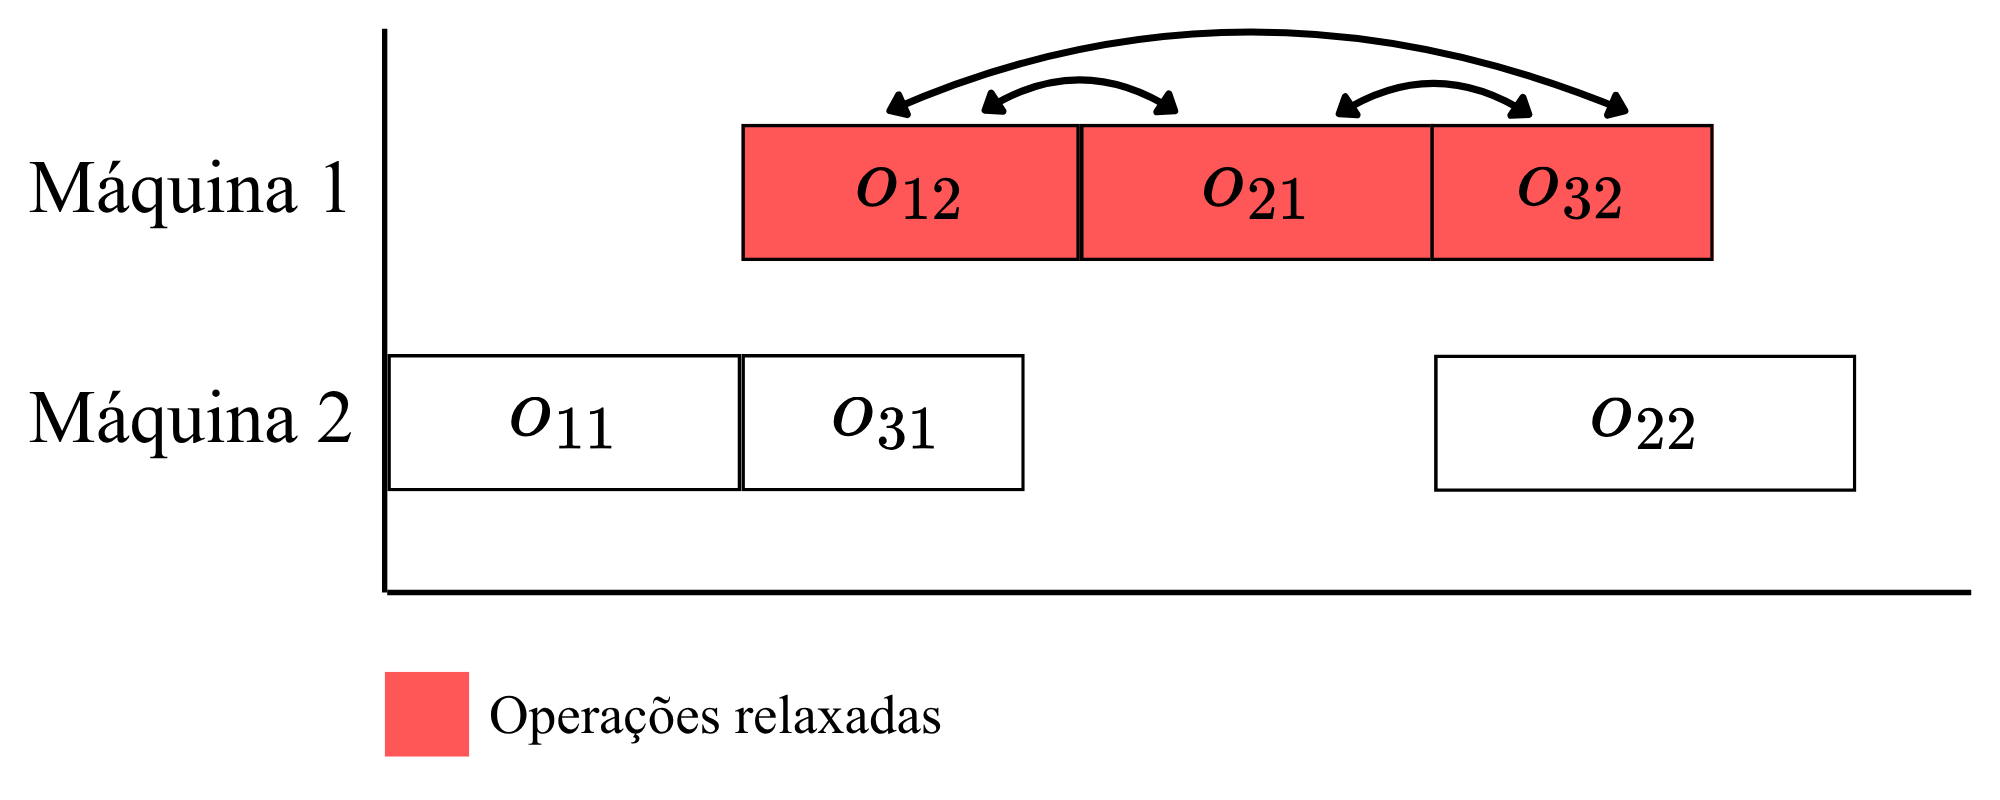
\includegraphics[width=\textwidth]{img/relax_a.png}
         \caption{Agendamento com subconjunto das operações relaxadas pela vizinhança.}
         \label{img:exemplo_relax_a}
     \end{subfigure}
     \hfill
     \begin{subfigure}[b]{0.45\textwidth}
         \centering
         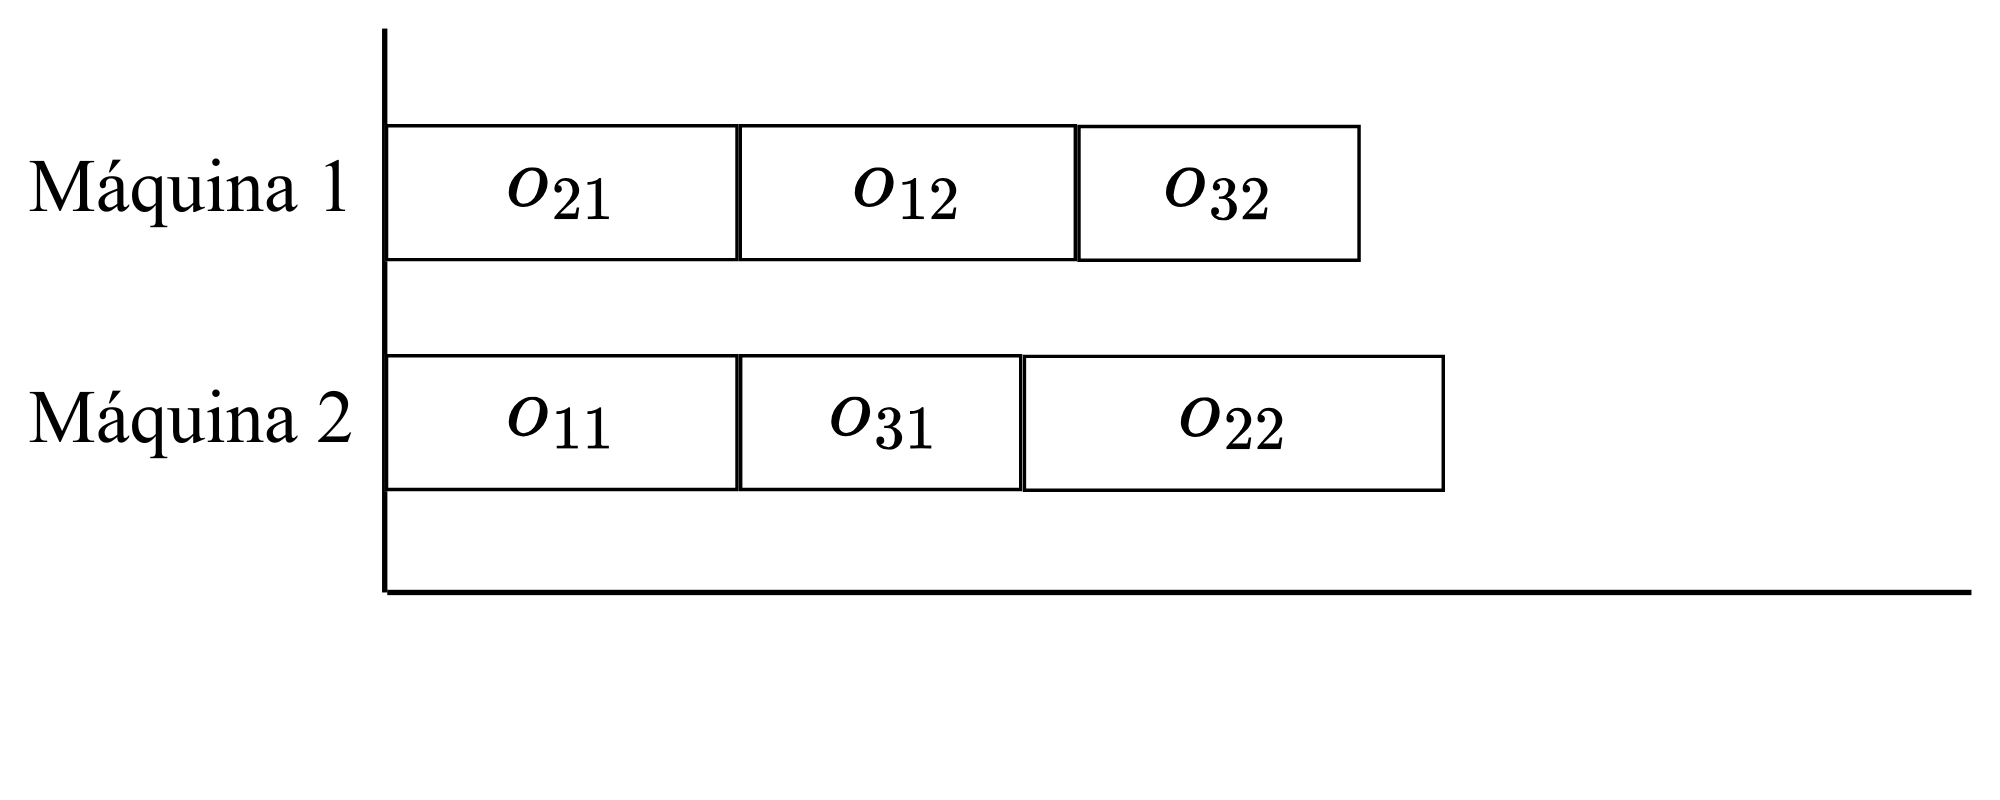
\includegraphics[width=\textwidth]{img/relax_b.png}
         \caption{Agendamento após a reordenação das operações relaxadas.}
         \label{img:exemplo_relax_b}
     \end{subfigure}
     \caption*{Fonte: adaptado de \cite{ahmadian2021meta}}
\end{figure}

A Figura \ref{img:exemplo_relax} ilustra o processo de otimização realizado por este método. No exemplo da Figura \subref{img:exemplo_relax_a}, o algoritmo relaxa a ordem de três operações, permitindo que o solver CPLEX explore qualquer permutação entre elas. Nesse caso, como representado na figura \subref{img:exemplo_relax_b}, as operações são reorganizadas e, por conta disso, todas as operações de ambas as máquinas são adiantadas. 

O projeto divide as demais vizinhanças implementadas em dois grupos: troca e remoção-inserção. As vizinhanças de troca realizam a troca de posição entre duas operações. Já as vizinhanças de remoção-inserção removem uma operação da sua posição e inserem em outra posição da sequência. Recapitulando a Seção \ref{sect:grafo_disj}, restrições de máquina limitam esses deslocamentos estritamente entre operações processadas na mesma máquina.

\begin{figure}[h!]
     \centering
     \caption{Exemplos dos dois tipos principais de vizinhanças: troca e remoção-inserção.}
     \label{fig:exemplos_swap_insert}
     \begin{subfigure}[b]{0.48\textwidth}
         \centering
         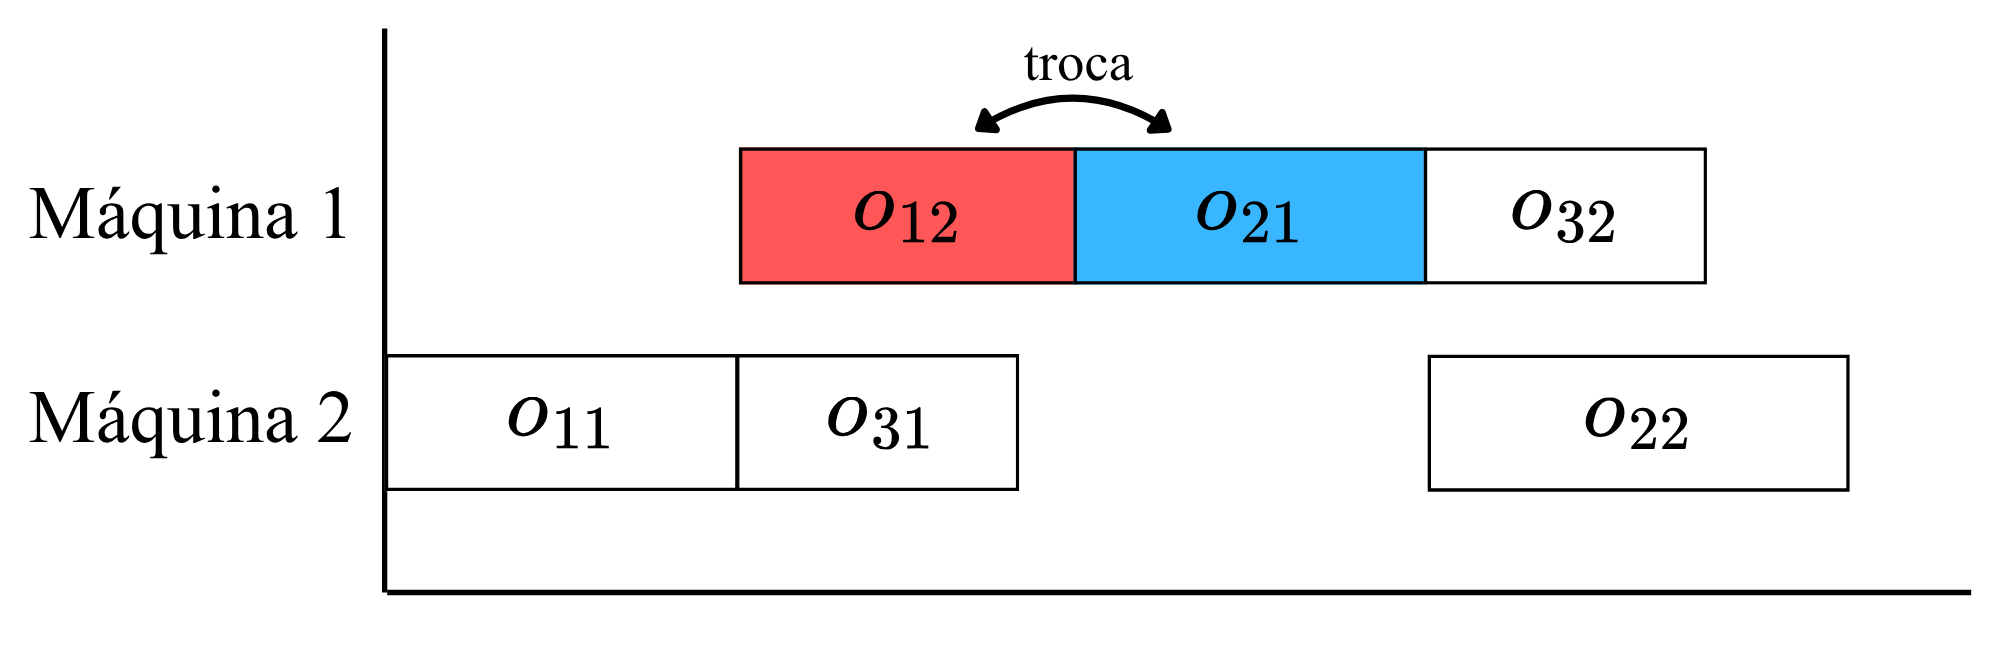
\includegraphics[width=\textwidth]{img/swap_insert_a.png}
         \caption{Agendamento antes de acontecer troca entre $o_{12}$ e $o_{21}$}
         \label{img:exemplos_swap_insert_a}
     \end{subfigure}
     \hfill
     \begin{subfigure}[b]{0.48\textwidth}
         \centering
         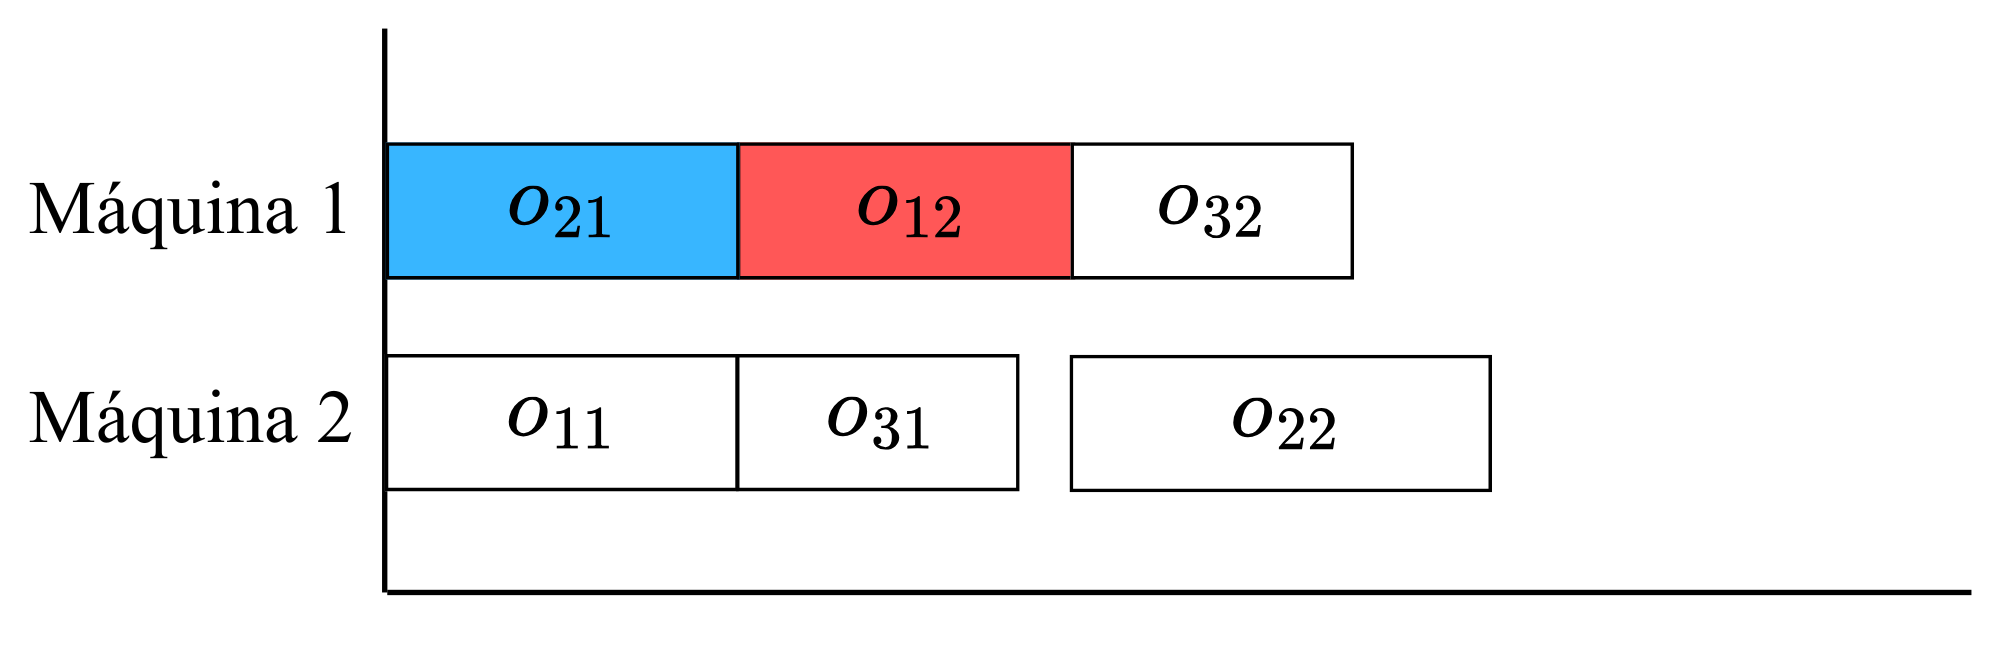
\includegraphics[width=\textwidth]{img/swap_insert_b.png}
         \caption{Agendamento após a troca entre $o_{12}$ e $o_{21}$.}
         \label{img:exemplos_swap_insert_b}
     \end{subfigure}
     
     \vspace{0.5em} % Espaçamento entre as linhas de figuras

     \begin{subfigure}[b]{0.48\textwidth}
         \centering
         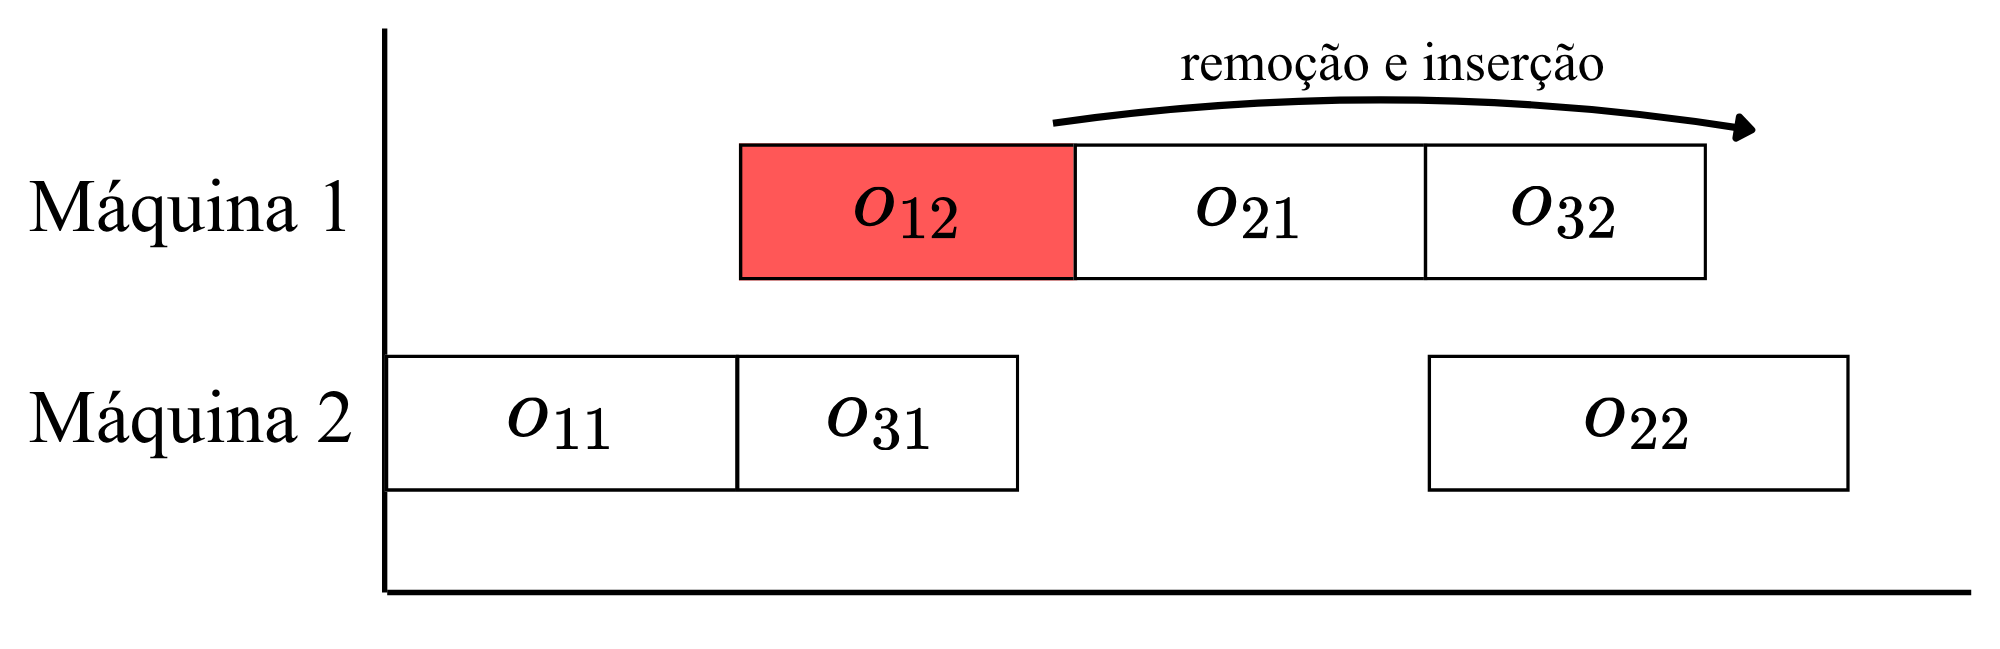
\includegraphics[width=\textwidth]{img/swap_insert_c.png}
         \caption{Agendamento antes de acontecer remoção e inserção de $o_{12}$.}
         \label{img:exemplos_swap_insert_c}
     \end{subfigure}
     \hfill
     \begin{subfigure}[b]{0.48\textwidth}
         \centering
         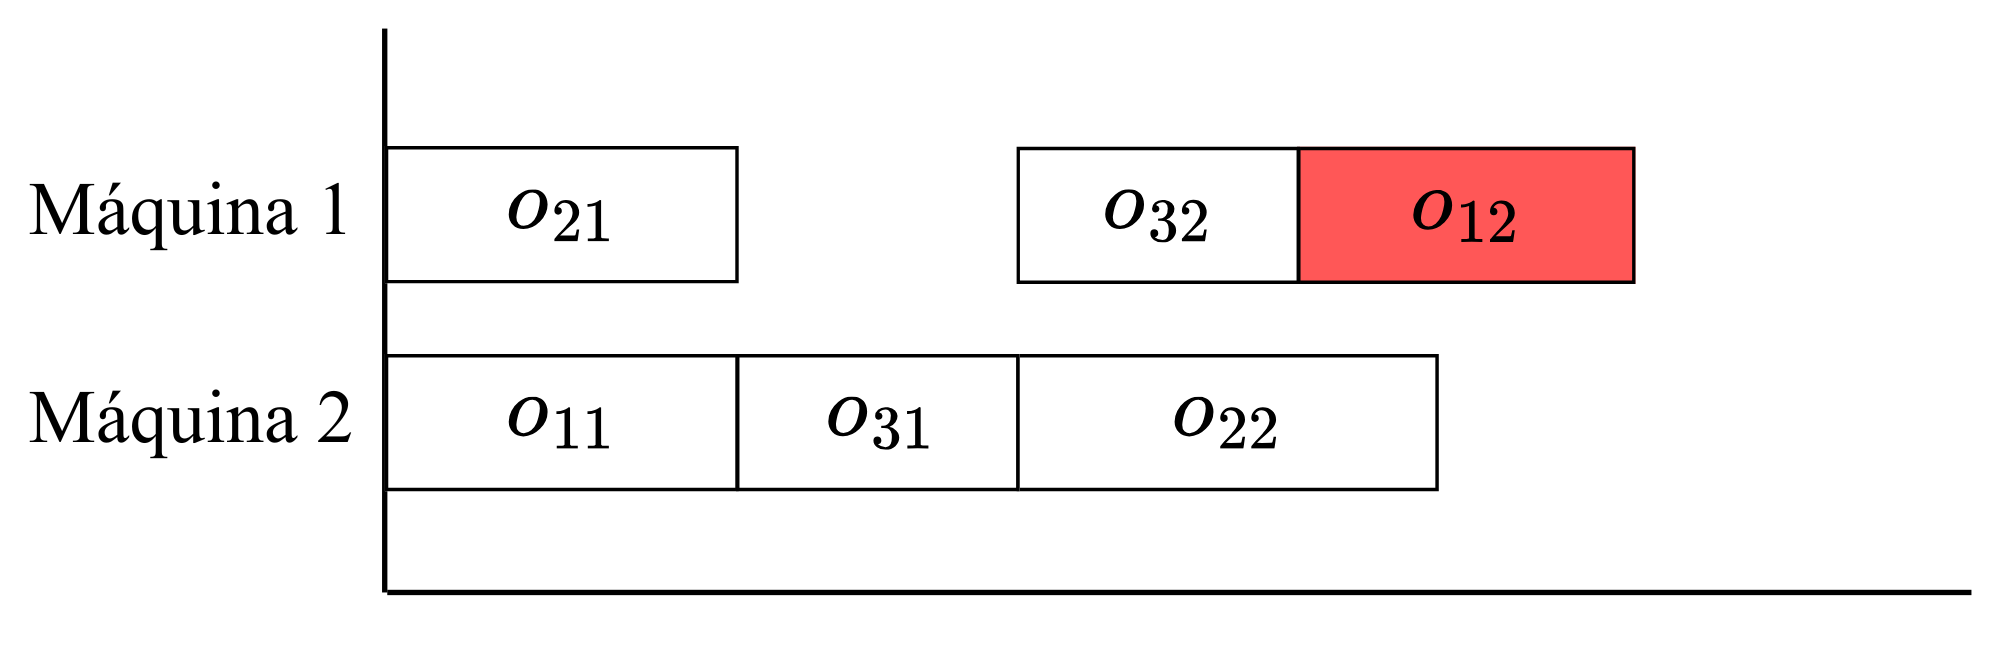
\includegraphics[width=\textwidth]{img/swap_insert_d.png}
         \caption{Agendamento após remoção-inserção com $o_{12}$ no final de uma máquina.}
         \label{img:exemplos_swap_insert_d}
     \end{subfigure}
     \caption*{Fonte: os autores.}
\end{figure}

A Figura \ref{fig:exemplos_swap_insert} apresenta exemplos práticos de ambos os tipos de movimentos. As figuras \subref{img:exemplos_swap_insert_a} e \subref{img:exemplos_swap_insert_b} demonstram a execução de uma troca no agendamento. Já as figuras \subref{img:exemplos_swap_insert_c} e \subref{img:exemplos_swap_insert_d} demonstram a execução de uma remoção de uma operação e inserção em outra posição do agendamento.

Primeiramente, temos as vizinhanças aleatórias utilizadas no trabalho de \cite{ahmadian2021meta}. Uma delas seleciona duas operações aleatoriamente e realiza a troca de posição entre as duas operações, e a outra remove uma operação aleatória e a insere em outra posição aleatória. Chamaremos a primeira de \texttt{troca\_al} e a segunda de \texttt{insere\_al}.

A fundamentação das próximas vizinhanças exige a formalização de definições preliminares. Definimos operações adjacentes entre si como aquelas que não possuem nenhum tempo ocioso entre elas. Dada uma operação $o$, a antecessora e a sucessora de tarefa de $o$ são, respectivamente, as operações que ocorrem antes e depois da operação $o$ dentro da ordem da tarefa de $o$. De forma similar, em uma sequência definida, a antecessora e a sucessora de máquina de $o$ são, respectivamente, as operações que são processadas antes e depois de $o$ na mesma máquina. A notação estabelece $JA(o)$ e $JS(o)$ como a antecessora e sucessora de tarefa, respectivamente, da operação $o$, que também são adjacentes a $o$. Da mesma forma, definimos $MA(o)$ e $MS(o)$, respectivamente, como a antecessora e sucessora de máquina da operação $o$ que também são adjacentes a $o$. Por fim, ao nos referirmos a um bloco de operações, considere um conjunto de operações adjacentes em uma mesma máquina.

A próxima vizinhança possui uma estrutura simplificada. Este componente provém do trabalho de \cite{dos2010combination} e realiza a troca de posição entre uma operação e sua sucessora de máquina, sem nenhum tipo de filtro. Partindo de qualquer solução, essa vizinhança gera sempre um número fixo de vizinhos e contém todas as outras vizinhanças que realizam trocas entre operações adjacentes com algum tipo de filtro. A nomenclatura \texttt{troca\_adj} identifica esta vizinhança.

O trabalho de \cite{wang2014variable} fundamenta outras duas vizinhanças que são baseadas nas penalidades das operações. A vizinhança de troca baseia-se no seguinte lema. Se uma operação $o$ está atrasada, $MA(o)$ não existe e $JA(o)$ existe, então $JA(o)$ também está atrasada. E, no caso inverso, se uma operação $o$ está adiantada, $MS(o)$ não existe e $JS(o)$ existe, então $JS(o)$ também está atrasada. Nesse sentido, a partir de uma operação $o$ adiantada (ou atrasada), o algoritmo percorre o agendamento seguindo as operações $JS(o)$ (ou $JA(o)$) até encontrar uma operação que possua uma $MS(o)$ (ou $MA(o)$) ou encontrar uma operação que seja a última (ou a primeira) operação da máquina ou da tarefa. A nomenclatura \texttt{troca\_penal} identifica esta vizinhança.

\begin{figure}[h!]
     \centering
     \caption{Exemplo de modificação de soluções pela vizinhança troca\_penal.}
     \label{img:exemplo_swap_penal}
     \begin{subfigure}[b]{0.45\textwidth}
         \centering
         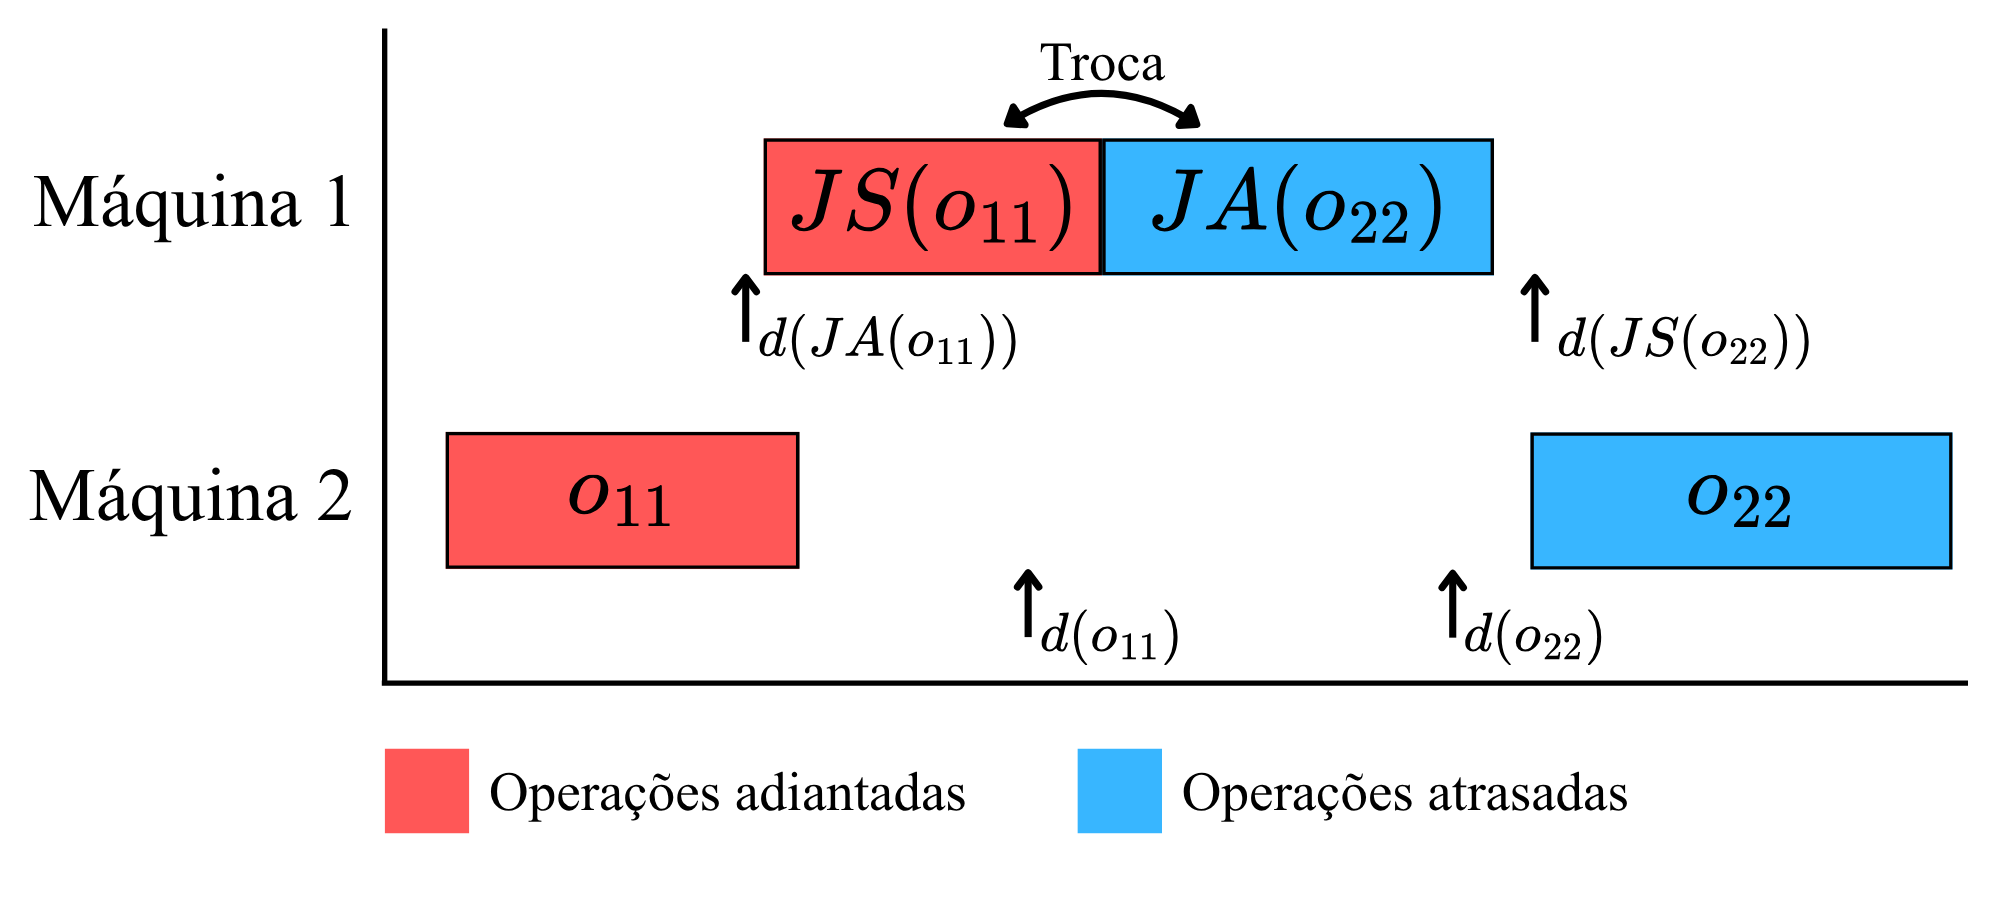
\includegraphics[width=\textwidth]{img/swap_penal_a.png}
         \caption{Agendamento com operações atrasadas e adiantadas com possível modificação pela vizinhança troca\_penal.}
         \label{img:exemplo_swap_penal_a}
     \end{subfigure}
     \hfill
     \begin{subfigure}[b]{0.45\textwidth}
         \centering
         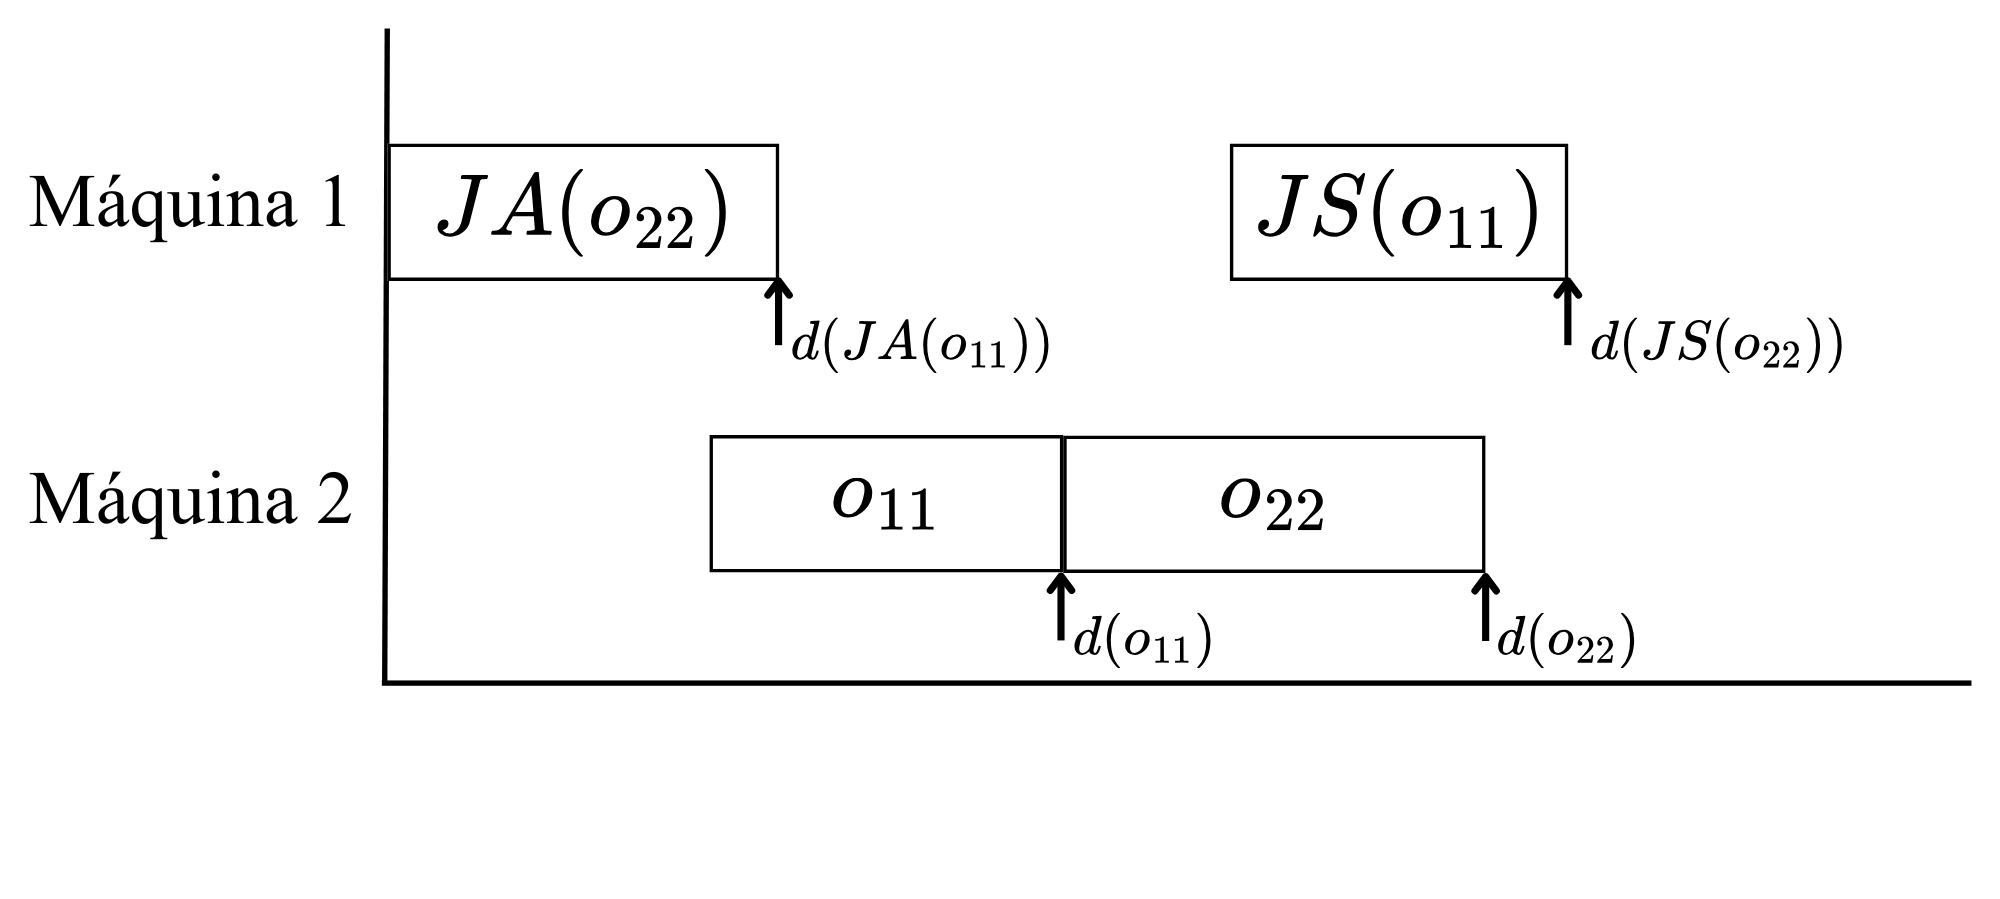
\includegraphics[width=\textwidth]{img/swap_penal_b.png}
         \caption{Agendamento após a modificação da vizinhança troca\_penal com todas as operações entregues nos seus prazo de entrega.}
         \label{img:exemplo_swap_penal_b}
     \end{subfigure} 
     \caption*{Fonte: Adaptado de \cite{wang2014variable}}
\end{figure}

Por exemplo, na Figura \ref{img:exemplo_swap_penal} podemos observar um exemplo de aplicação desta vizinhança. A partir da operação adiantada $o_{11}$, ao seguir a sucessora $JS(o_{11})$, o procedimento localiza uma troca capaz de zerar as penalidades de todas as operações envolvidas. De forma semelhante, a partir da operação atrasada $o_{22}$, seguindo a antecessora $JA(o_{22})$, o algoritmo encontraria a mesma troca. 

No caso da vizinhança de remoção-inserção baseada nas penalidades, se uma operação está adiantada, a vizinhança remove a operação e tenta inseri-la ao final do bloco correspondente. Por outro lado, se uma operação está atrasada, a vizinhança a remove e tenta inseri-la no início do bloco. Todo o procedimento condiciona a inserção ao agendamento atual para preservar a localidade do movimento. Para uma operação adiantada $o$ que seria inserida ao final do bloco, se o tempo de término do bloco for maior que o tempo de início da sucessora de tarefa de $o$, então $o$ é inserida após a primeira operação do bloco que possui tempo de término menor que o tempo de início de sua sucessora de tarefa. Da mesma maneira, para uma operação atrasada que seria inserida no início do bloco, se o tempo de início do bloco for menor que o tempo de término da antecessora de tarefa de $o$, então $o$ será inserida antes da primeira operação do bloco que possuir tempo de início maior que o tempo de término da sua antecessora. A nomenclatura \texttt{insere\_penal} identifica esta vizinhança.

A Figura \ref{fig:exemplos_insert_penal_earl} ilustra como essa modificação acontece, juntamente com o mecanismo de controle do impacto das modificações. Nessa figura, a operação $u$ está adiantada e a vizinhança tentaria inseri-la no fim do seu bloco, isto é, após a operação $w$. No primeiro cenário, nas figuras \subref{img:exemplos_insert_penal_earl_a} e \subref{img:exemplos_insert_penal_earl_b}, $JS(u)$ tem um tempo de início maior que o término do bloco, ou seja, inserir $u$ no fim do bloco não afetaria o tempo de inicio de sua sucessora, então, o movimento acontece. Já no segundo cenário, nas figuras \subref{img:exemplos_insert_penal_earl_c} e \subref{img:exemplos_insert_penal_earl_d}, inserir $u$ no fim do bloco não é possível sem atrasar sua sucessora. Por isso, a inserção é realizada antes da operação $w$, mantendo a posição anterior de $JS(u)$. Quando nossa operação alvo está atrasada, esse processo acontece de forma similar, porém observando os critérios descritos no parágrafo anterior.

\begin{figure}[h!]
     \centering
     \caption{Exemplos das modificações da vizinhança insere\_penal para um operação adiantada.}
     \label{fig:exemplos_insert_penal_earl}
     \begin{subfigure}[b]{0.48\textwidth}
         \centering
         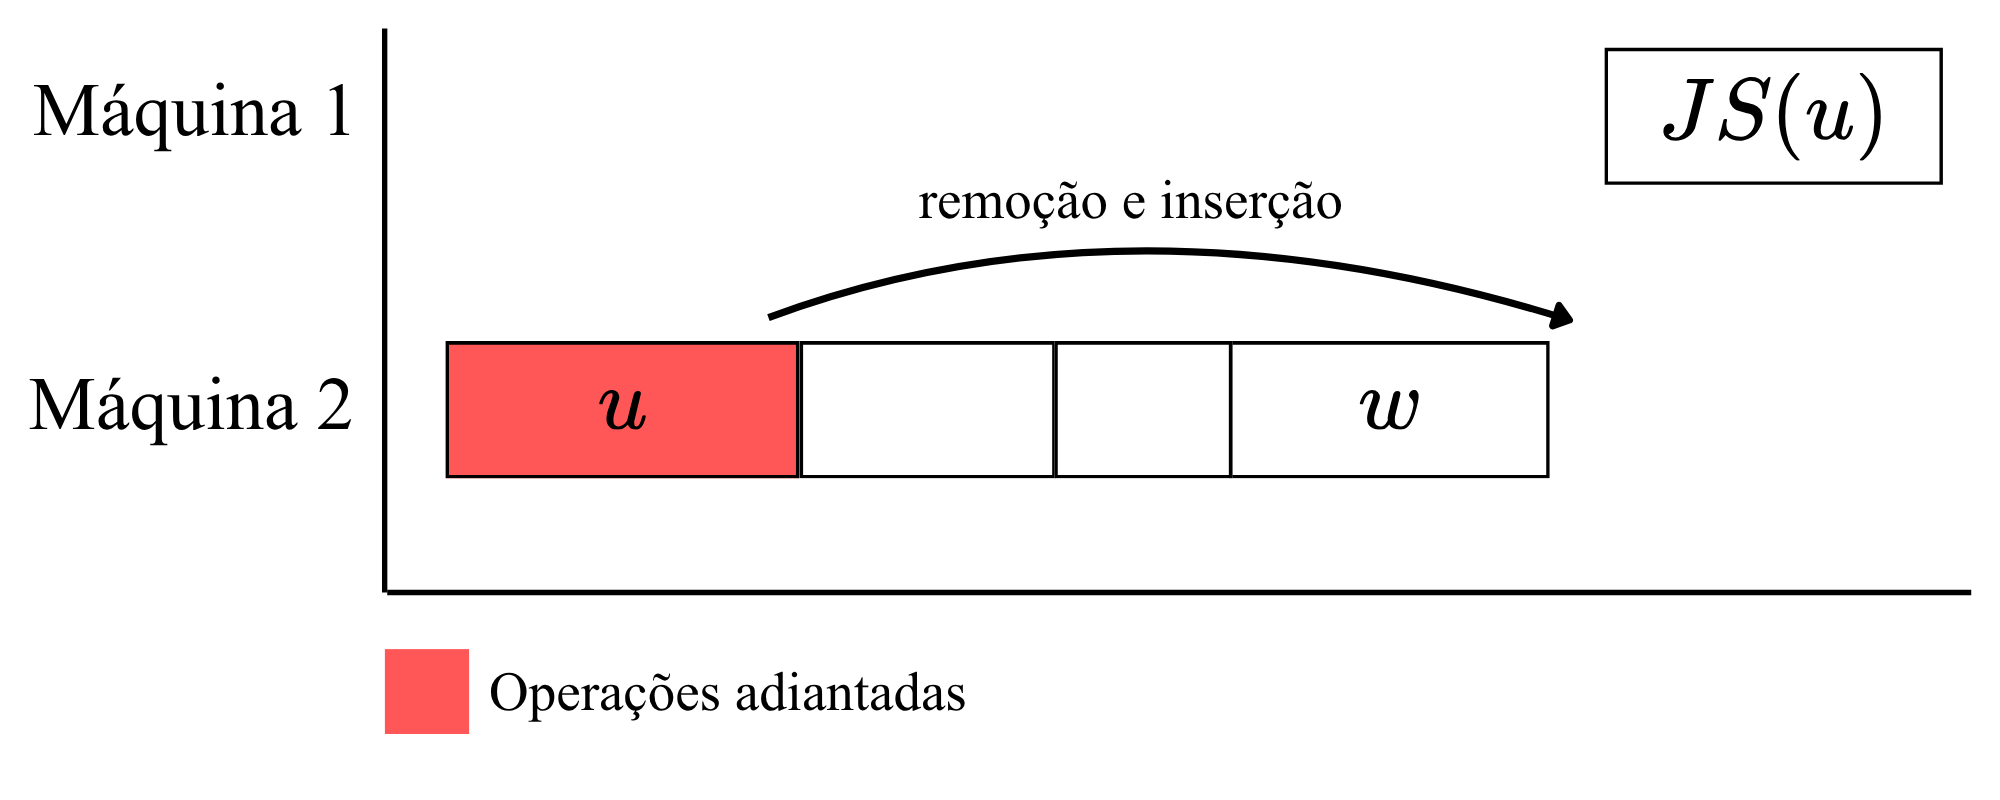
\includegraphics[width=\textwidth]{img/insert_penal_earl_a.png}
         \caption{Agendamento com operação $u$ adiantada e tempo de início de $JS(u)$ maior que tempo de término do bloco.}
         \label{img:exemplos_insert_penal_earl_a}
     \end{subfigure}
     \hfill
     \begin{subfigure}[b]{0.48\textwidth}
         \centering
         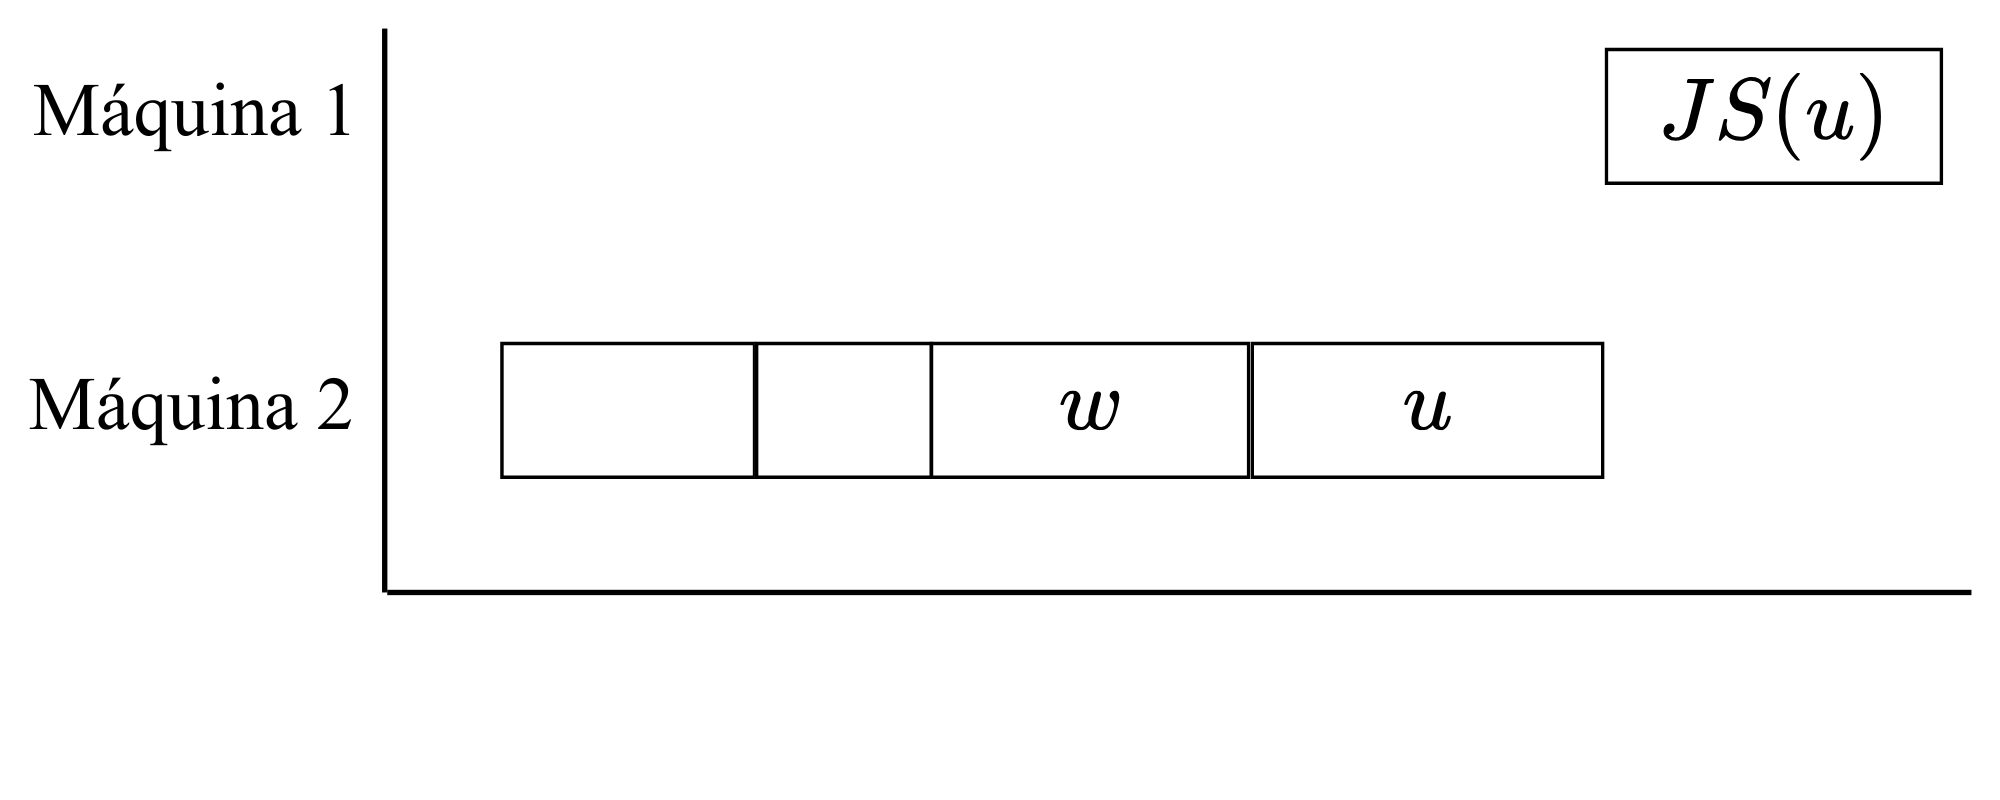
\includegraphics[width=\textwidth]{img/insert_penal_earl_b.png}
         \caption{Agendamento após inserção de $u$ no fim do bloco tendo sua penalidade de adiantamento reduzida.}
         \label{img:exemplos_insert_penal_earl_b}
     \end{subfigure}
     
     \vspace{0.3em} % Espaçamento entre as linhas de figuras

     \begin{subfigure}[b]{0.48\textwidth}
         \centering
         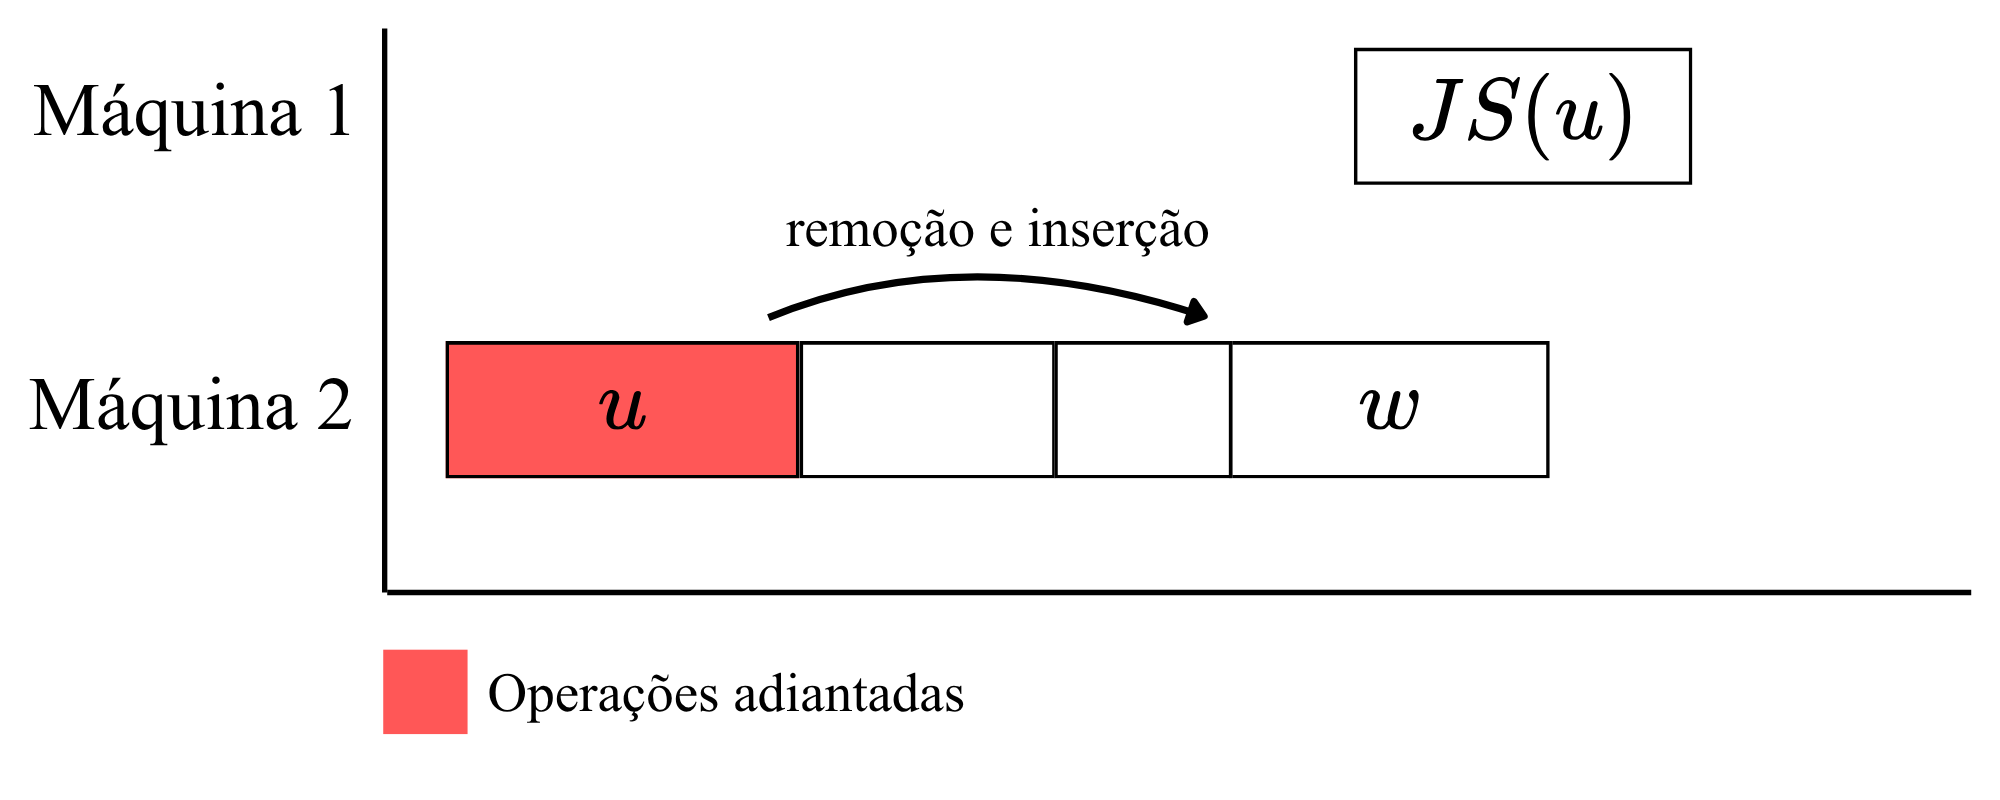
\includegraphics[width=\textwidth]{img/insert_penal_earl_c.png}
         \caption{Agendamento com operação $u$ adiantada e tempo de início de $JS(u)$ menor que tempo de término do bloco.}
         \label{img:exemplos_insert_penal_earl_c}
     \end{subfigure}
     \hfill
     \begin{subfigure}[b]{0.48\textwidth}
         \centering
         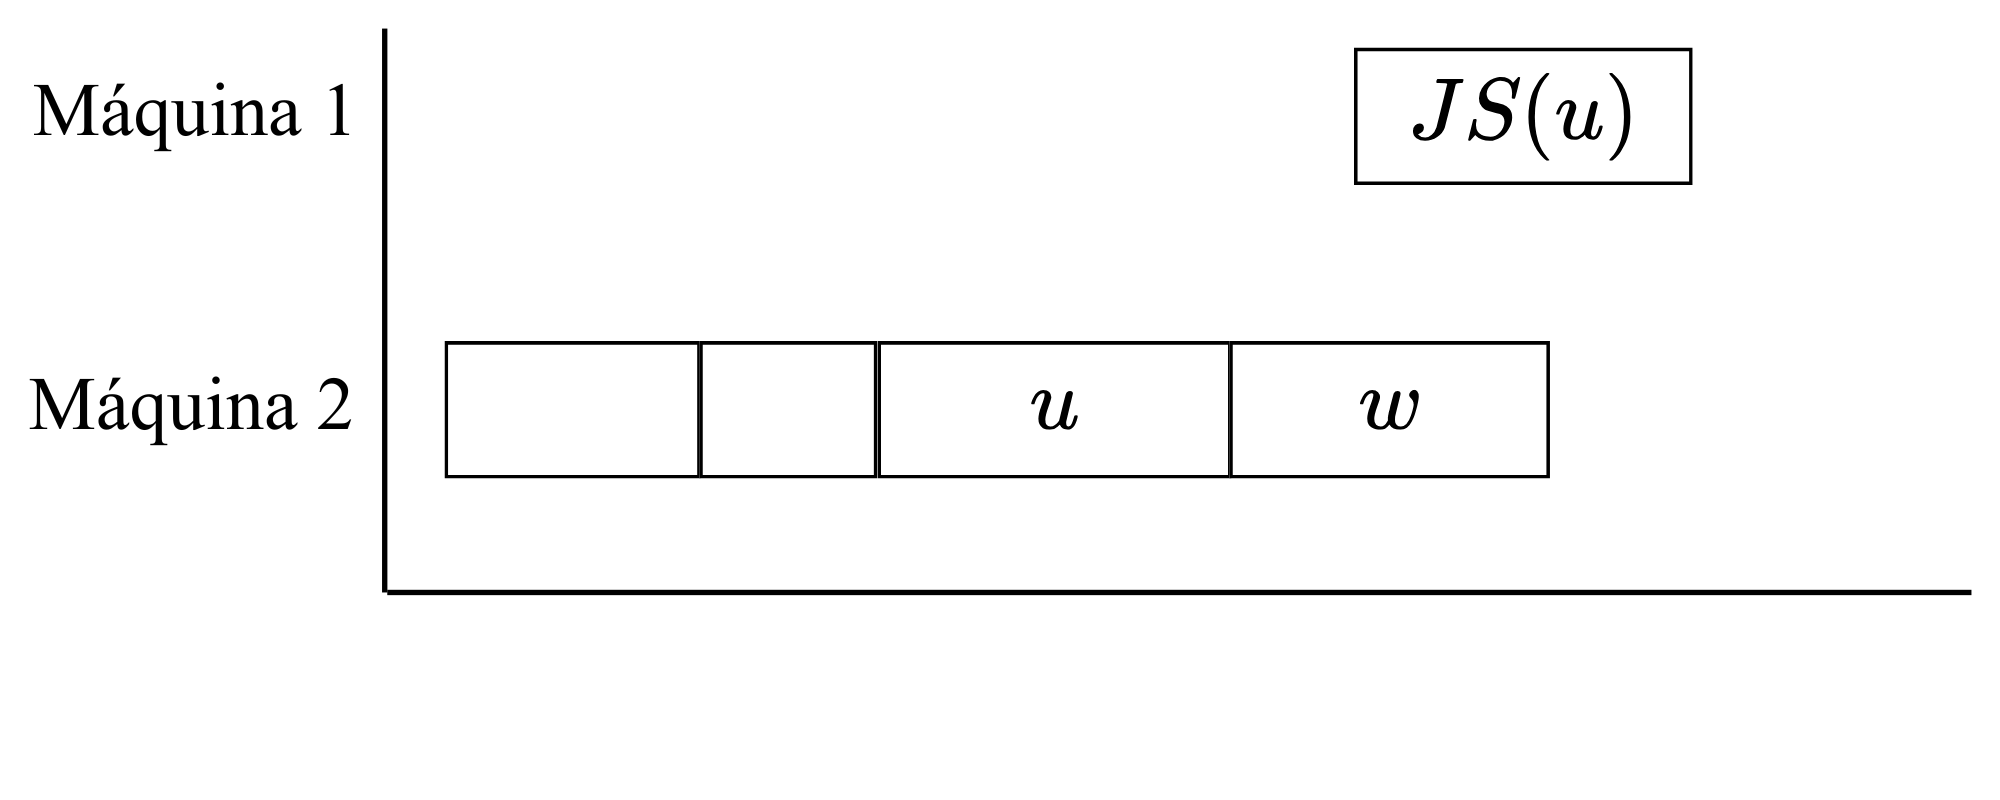
\includegraphics[width=\textwidth]{img/insert_penal_earl_d.png}
         \caption{Agendamento após inserção de $u$ no meio do bloco ainda tendo sua penalidade de adiantamento reduzida.}
         \label{img:exemplos_insert_penal_earl_d}
     \end{subfigure}
     \caption*{Fonte: adaptado de \cite{wang2014variable}.}
\end{figure}

Por fim, este trabalho propõe uma vizinhança original ao \ac{JITJSS}, fundamentada na estrutura N5 de \cite{nowicki1996fast} para o problema \ac{JSS}, mas adaptada para a redução de penalidades por atraso. Os autores propõem uma vizinhança que explora o conceito explicado na Seção \ref{sect:grafo_disj} de que apenas alterações no caminho crítico de um agendamento alteram seu \textit{makespan}. Nesse sentido, a vizinhança consiste em realizar a troca de posição entre as duas primeiras e as duas últimas operações de cada um dos blocos críticos do agendamento, isto é, blocos de operações que estão contidos no caminho crítico. Perceba que a ideia da otimização do \textit{makespan} é adiantar o tempo de início da última operação do caminho crítico.

% \begin{figure}[h!] 
%     \centering 
%     \caption{Exemplo da vizinhança RELAX}
%     \label{img:exemplo_viz_insert_penal_tard}
%     \includegraphics[width=0.9\linewidth]{img/insert_penal_tard.png}
%     \caption*{\small \textbf{Fonte:} Os Autores.}
% \end{figure}

Dessa forma, a vizinhança proposta aplica o conceito de caminho crítico individualmente para cada uma das operações atrasadas do agendamento. Para isso, dada uma operação $o$ atrasada, o algoritmo compõe o caminho crítico ao percorrer as antecessoras de $o$ de forma iterativa. A cada iteração, a nova operação a ser adicionada no caminho crítico será a operação com o maior tempo de término entre $JA(o)$ e $MA(o)$, isto é, a operação que impede a operação atual de ser adiantada. A construção do caminho crítico de $o$ termina após encontrar uma operação que não possui nem $JA$ nem $MA$. A posse desse caminho crítico permite ao algoritmo gerar vizinhos da solução original por meio da estrutura N5. A nomenclatura \texttt{troca\_crit} identifica esta vizinhança.

\begin{figure}[h!] 
    \centering 
    \caption{Exemplo de modificações vizinhas geradas pela vizinhança troca\_crit.}
    \label{img:exemplo_viz_critical}
    
\includegraphics[width=0.75\linewidth]{img/oper_crit.png}
    \caption*{\small \textbf{Fonte:} Os Autores.}
\end{figure}

A Figura \ref{img:exemplo_viz_critical} apresenta um cenário no qual a operação $o_{12}$ está atrasada, isto é, reduzir seu tempo de início pode contribuir para a redução das penalidades. A aplicação da vizinhança \texttt{troca\_crit} exige a identificação do caminho crítico específico da operação em questão. A execução do processo descrito no parágrafo anterior resulta na identificação das operações destacadas em vermelho como o caminho crítico de $o_{12}$. Essas operações representam o caminho de dependência da operação $o_{12}$, e apenas a modificação delas é capaz de reduzir o tempo de início de $o_{12}$. A partir disso, esse caminho crítico gera três vizinhos a partir das trocas das operações $o_{11}$ com $o_{31}$, $o_{32}$ com $o_{21}$ e $o_{21}$ com $o_{12}$. Trocas estas que correspondem aos pares de operações nas extremidades de cada bloco crítico.

\subsection{Métodos de busca}

A exploração das vizinhanças a partir de uma solução inicial requer o emprego de métodos de busca heurística. Para isso, o projeto contempla três opções de métodos de busca: uma busca local simples conforme explicada na Seção \ref{sect:meta}, a busca tabu e a busca local iterada.

A busca tabu segue o que foi definido na seção \ref{sect:meta}, mas com a adição de mecanismos que melhoram a intensificação e a exploração do processo de busca. Primeiramente, precisamos definir como a lista tabu armazenará os movimentos que devem ser proibidos enquanto forem tabu. A estrutura de memória registra exclusivamente as arestas do grafo disjuntivo desfeitas pelas modificações na solução. Essa abordagem garante a representação universal de qualquer movimento, uma vez que o grafo disjuntivo sustenta todas as soluções do problema. O detalhe é que cada um dos tipos de modificações é armazenado de forma ligeiramente diferente.

Nas vizinhanças de troca entre duas operações, o algoritmo classifica as arestas de entrada das operações envolvidas como tabu. Por exemplo, se uma máquina possui a seguinte ordem de operações $o1 \xrightarrow{} o2 \xrightarrow{} o3 \xrightarrow{} o4 \xrightarrow{} o5$, então as arestas $\{(o1,o2),(o2,o3),(o3,o4), (o4,o5)\}$ existem no grafo disjuntivo. Se uma vizinhança realiza a troca de posição entre as operações $o2$ e $o4$, então as arestas $(o1,o2)$ e $(o3,o4)$ se tornam tabu. Isso impede, neste exemplo, o retorno das operações $o2$ e $o4$ às posições sucessoras de $o1$ e $o2$ durante a vigência do \textit{tenure}. 

Nas vizinhanças de remoção-inserção, apenas a aresta de entrada da operação removida é adicionada como tabu. No mesmo exemplo do parágrafo anterior, se a operação $o2$ for removida e inserida após $o3$, então a aresta $(o1,o2)$ se torna tabu. Com isso, $o2$ é impedida de retornar como sucessora de $o1$ nas próximas iterações.

A verificação da lista tabu acontece durante a exploração da vizinhança pela busca tabu. Durante esse processo, dada uma lista de opções de modificações geradas por uma vizinhança, o procedimento de busca avalia as modificações geradas e seleciona o movimento conforma a seguinte hierarquia de prioridade:

\begin{enumerate}
    \item A melhor modificação, seja ela tabu ou não, que seja menor que a melhor solução encontrada até o momento. Este item aplica o critério de aspiração na exploração da vizinhança.
    \item A melhor modificação que não seja tabu.
    \item A modificação mais antiga da lista tabu.
\end{enumerate}

Todo movimento escolhido é adicionado à lista tabu de acordo com seu tipo, conforme descrito anteriormente. Esse movimento continuará tabu durante um número de iterações determinado pelo \textit{tabu tenure}. A meta-heurística incrementa a contagem de tempo da lista a cada nova inserção. Além disso, caso o algoritmo selecione a modificação tabu mais antiga durante a exploração, o sistema adianta o relógio da lista até o instante em que tal movimento perderia a condição de tabu, removendo simultaneamente da lista elementos mais antigos. Por exemplo, se uma lista tabu possui \textit{tabu tenure} igual a 20 e $5$ elementos que foram adicionados há $2$, $7$, $12$, $14$ e $16$ iterações. Se a modificação com idade $12$ foi escolhida dentro de alguma vizinhança, as iterações da lista tabu serão avançadas em $8$, fazendo com que os elementos com mais idade que $12$ também saiam da lista tabu, restando dois elementos com idades de $10$ e $15$ iterações.

Além da lista tabu, a implementação integra dois mecanismos baseados no trabalho de \cite{zubaran2016tabu} para otimizar a exploração do espaço de busca: uma lista de soluções elite para intensificação e um detector de ciclos para evitar estagnação. A lista de elites $E$ contém as $L$ melhores soluções encontradas durante a busca. Quando uma nova solução gera melhoria, ela é adicionada a $E$. Caso $E$ esteja em sua capacidade máxima, a solução mais antiga é removida. Além disso, o sistema armazena, para cada entrada em $E$, o estado completo da busca, incluindo a lista de vizinhos que ainda não foram explorados e a configuração atual da lista tabu.

A busca inicia em uma solução inicial $s^*$ e explora as vizinhanças a partir dela por um orçamento de até $I$ iterações. O algoritmo reinicia o orçamento de iterações $I$ sempre que identifica uma melhoria na solução atual. Ao atingir o limite de iterações determinado por $I$, ou ao detectar um ciclo, a busca retoma a exploração a partir da solução elite mais recente, selecionando um de seus vizinhos ainda não explorados. Este movimento de diversificação aplica um fator de redução $F$ sobre o orçamento máximo $I$. Se nenhuma solução elite existir, a busca para.

Por fim, o detector de ciclos mencionado anteriormente consiste no armazenamento de uma lista de valores de soluções passadas. A partir disso, a busca tabu verifica a repetição desses valores objetivos a cada iteração. Caso essa repetição ocorra mais do que um número máximo de vezes, um ciclo é detectado e o processo descrito no parágrafo anterior é executado.

O terceiro método de busca no espaço de projeto consiste na busca local iterada. Como descrita na Seção \ref{sect:meta}, ela é capaz de utilizar internamente tanto a busca local quanto a busca tabu como heurísticas de busca. Ao utilizar a busca local, ela se comporta como uma \ac{ILS} comum, e ao utilizar a busca tabu, ela se comporta como uma busca tabu iterada. A cada iteração da \ac{ILS}, ela realiza uma perturbação na solução base. Nesse sentido, o algoritmo utiliza a estratégia de perturbação proposta por \cite{ahmadian2021meta}. Ela consiste em escolher duas máquinas aleatoriamente e relaxar as restrições de precedência das máquinas em diversas operações. Dessa forma, o procedimento submete o modelo relaxado ao solver CPLEX com um limite de tempo de 1 segundo, permitindo que a ferramenta reorganize as operações e gere uma nova configuração inicial para a próxima busca local. gerando uma nova solução modificada.

Além disso, considerando que o atual estado da arte para o \ac{JITJSS} é um \ac{VNS}, a estrutura da \ac{ILS} admite a integração de uma coleção de vizinhanças, operando de forma análoga ao \ac{VNS}. Nesse âmbito, a meta-heurística respeita a ordem de entrada das vizinhanças durante a exploração do espaço de busca. A cada iteração sem melhora, a busca realiza uma perturbação e tenta utilizar a próxima vizinhança da lista em busca de melhorias na solução. Caso aconteça alguma melhoria na solução ou caso a coleção de vizinhanças chegue ao fim sem nenhuma melhora, a busca reinicia o ciclo das vizinhanças. Ademais, o espaço de projeto permite a alternância entre os critério de melhor melhora ou primeira melhora para cada vizinhança integrante da lista.

Ambos os métodos, busca local e busca tabu, são capazes de executar a exploração das vizinhanças sob os critérios de melhor melhora ou primeira melhora, com a única exceção sendo a vizinhança \texttt{relax}. No caso da exploração por primeira melhora, os movimentos candidatos são todos gerados e embaralhados aleatoriamente com o objetivo de remover algum viés causado pela ordem da geração dos vizinhos. Além disso, uma limitação importante é que a busca tabu não é capaz de utilizar a vizinhança \texttt{relax}. Visto que o solver realiza a sua própria exploração da vizinhança, a busca tabu perde visibilidade sobre as transições individuais de estados e, por isso, não consegue montar suas estruturas de intensificação e diversificação.

\subsection{Agendadores}

A avaliação da qualidade de uma sequência exige métodos de agendamento precisos, conforme discutido na Seção \ref{sect:grafo_disj}. Nesse sentido, a literatura do \ac{JITJSS} recorre frequentemente à programação inteira para converter sequências em agendamentos (Seção \ref{sect:bibjitjsp}). Por isso, o espaço de projeto contempla esta abordagem por meio da integração com o solver CPLEX. O modelo submetido ao solver fixa a ordem das máquinas e permite ao solver apenas determinar as posições temporais de cada operação.

O projeto integra, adicionalmente, um algoritmo de agendamento utilizado na minimização do \textit{makespan} no problema \ac{JSS}. Esse algoritmo consiste em agendar as operações o mais cedo possível, com complexidade linear. Porém, como discutido na Seção \ref{sect:grafo_disj}, essa forma de agendamento tende a gerar penalidades de adiantamento desnecessárias. Para mitigar esse efeito, o sistema adota a lógica de \cite{ferreira2023}. Após realizar o agendamento da forma descrita, o algoritmo percorre a solução, atrasando operações adiantadas que possuem tempo ocioso subsequente. O algoritmo restringe esse deslocamento a cenários que não impactam operações no prazo ou em atraso, garantindo que o procedimento preserve ou melhore o valor da função objetivo em todos os casos.

\section{Configuração automática} \label{sect:confauto}

Como proposto na metodologia e descrito no referencial teórico, agora que temos o espaço de projeto construído, precisamos formalizá-lo de forma que seja possível parametrizar a geração automática de algoritmos. Para isso, utilizaremos uma gramática livre de contexto.

\subsection{Gramática e parâmetros}

A Figura \ref{img:gramatica_final} contém a gramática que gera todas as combinações algorítmicas que o espaço de projeto admite. Todas as meta-heurísticas precisam de uma solução inicial (\texttt{sol\_ini}), que pode ser o algoritmo de \ac{GT} (\texttt{gt}) ou o algoritmo construtivo comum (\texttt{constr}). Ambas as soluções iniciais precisam de uma regra de despacho (\texttt{regra\_desp}) que pode ser aleatória (\texttt{aleatoria}), a \ac{EDD} (\texttt{edd}) ou a regra ALL+CR+SPT (\texttt{acs}).

\begin{figure}[h!] 
    \centering 
    \caption{Gramática livre de contexto para geração dos algoritmos}
    \label{img:gramatica_final}
    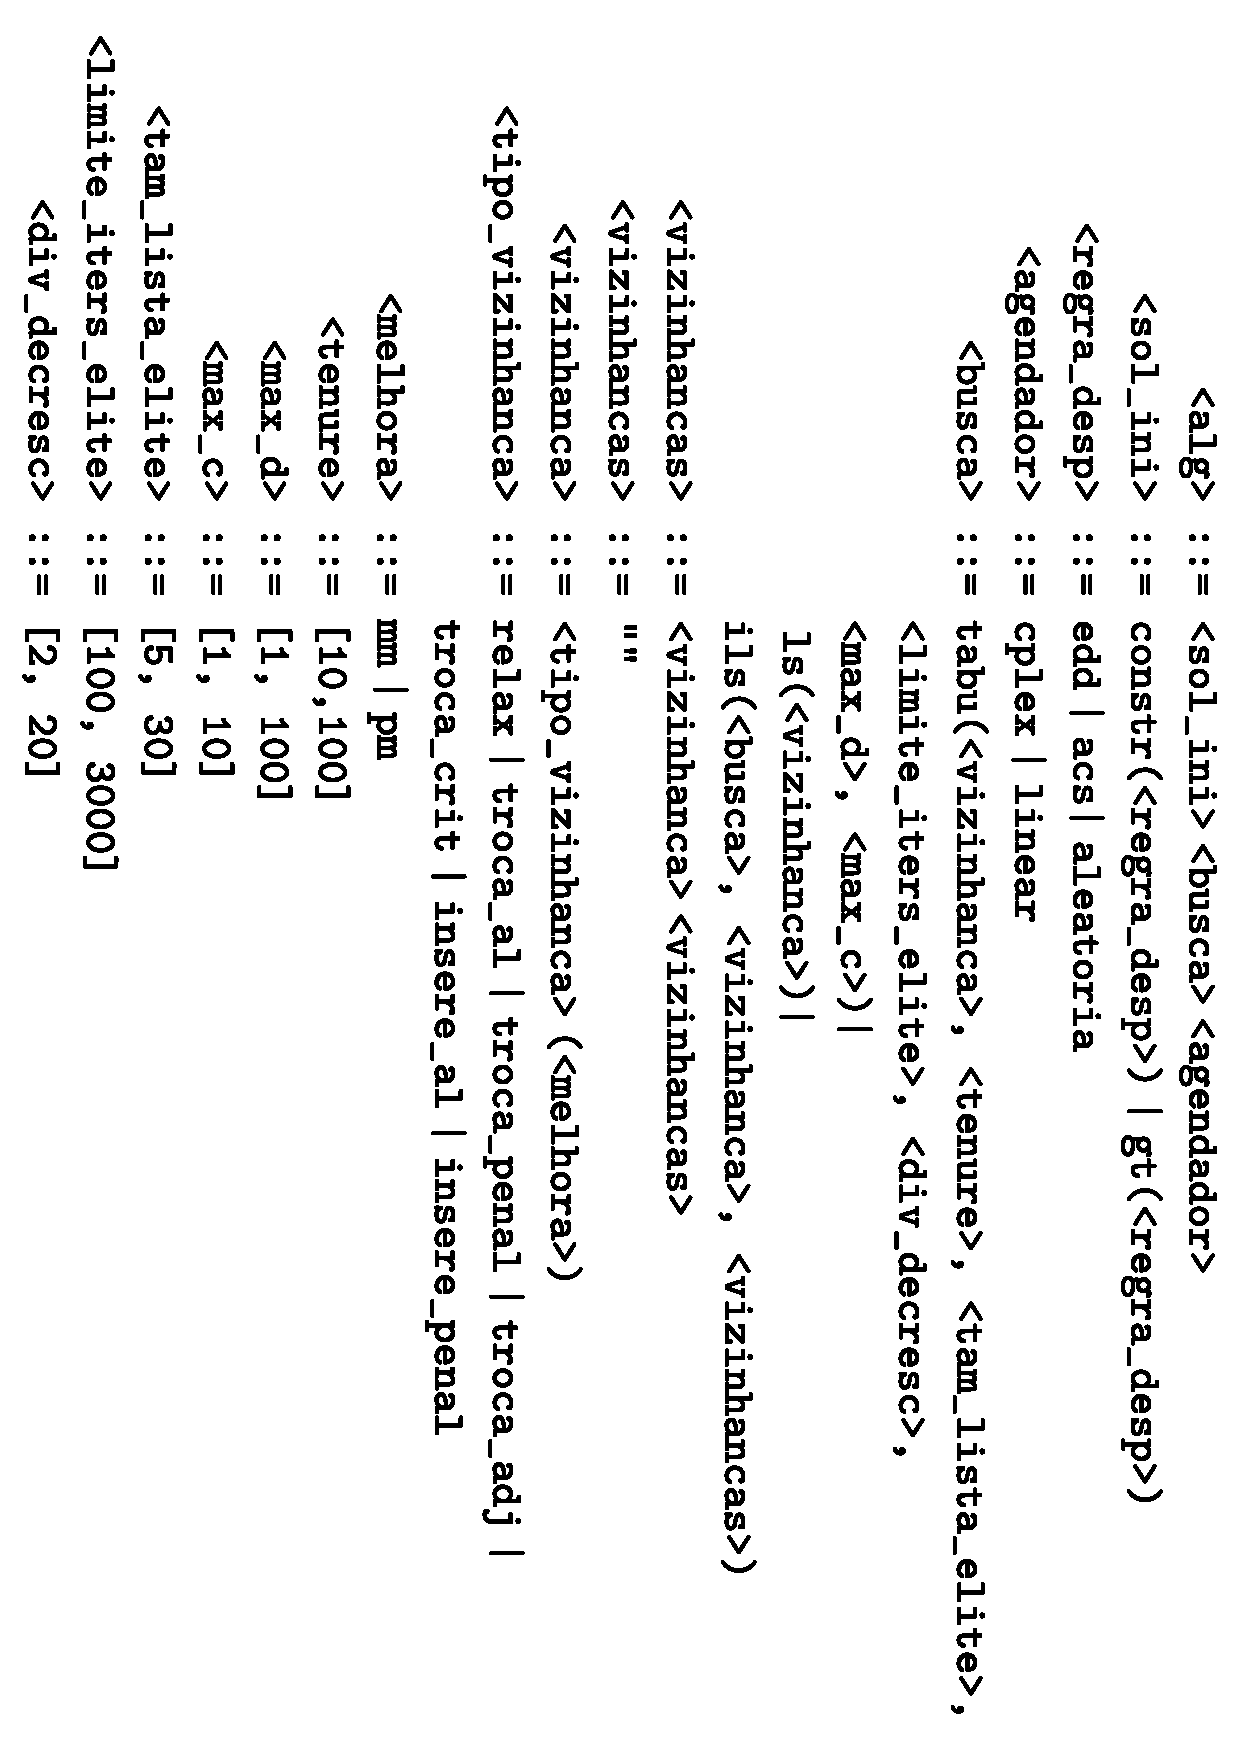
\includegraphics[angle=90, width=0.9\linewidth]{img/grammar.pdf}
    \caption*{\small \textbf{Fonte:} Os Autores.}
\end{figure}

Outro símbolo que independe das meta-heurísticas selecionadas é o agendador (\texttt{agendador}) para que o algoritmo seja capaz de avaliar a qualidade das sequências. O algoritmo é capaz de realizar este processo por meio de programação inteira (\texttt{cplex}) ou via procedimento linear que agenda as operações o mais cedo possível, mas com atraso deliberado para mitigação de penalidades de adiantamento (\texttt{linear}).

Após a derivação da solução inicial, da regra de despacho e do agendador, a gramática induz a escolha do método de busca (\texttt{busca}). Este pode ser uma \ac{LS} (\texttt{ls}), uma \ac{TS} (\texttt{tabu}) ou uma \ac{ILS} (\texttt{ils}). Os métodos de busca \texttt{ls} e \texttt{tabu} precisam apenas de uma vizinhança, que pode ser escolhida entre a \texttt{relax}, \texttt{troca\_al}, \texttt{troca\_penal}, \texttt{troca\_adj}, \texttt{troca\_crit}, \texttt{insere\_al} e \texttt{insere\_penal}. Por outro lado, a \texttt{ils} pode receber um número arbitrário de vizinhanças, e cada uma pode ser explorada por primeira melhora (\texttt{pm}) ou melhor melhora (\texttt{mm}).

A escolha do \texttt{tabu} como método de busca exige a definição de símbolos adicionais, como o tamanho da lista tabu (\texttt{tenure}). Os parâmetros da lista de elementos elite: o tamanho da lista (\texttt{tam\_list\_elite}), o número máximo de iterações para que um elemento da lista seja recuperado (\texttt{limite\_iters\_elite}) e o número que divide o limite de iterações quando nenhuma melhoria é encontrada (\texttt{div\_decresc}). Já o detector de ciclos requer o ajuste do tamanho do ciclo (\texttt{max\_d}) e do limite de repetições do mesmo ciclo para identificação de estagnação (\texttt{max\_c}).

Por fim, se escolhermos a \texttt{ils} como processo de busca, é necessário selecionar outro método de busca para ser utilizado internamente. Este caráter recursivo obriga o sistema a derivar novos símbolos idênticos aos anteriores até a obtenção de uma sequência de terminais formando um algoritmo executável.

Porém, como descrito na Seção \ref{sect:bottomup}, não podemos utilizar a gramática da Figura \ref{img:gramatica_final} em um algoritmo configurador, pois essa gramática gera infinitas palavras e o algoritmo configurador espera um espaço de projeto finito. Dessa forma, a realização da configuração automática exige uma conversão dessa gramática para um conjunto de parâmetros que force a finitude do espaço de projeto. A Tabela \ref{tab:irace_parameters} detalha o resultado da conversão. Em relação à gramática, os parâmetros representam símbolos não terminais que precisam ser derivados para os possíveis valores. Além disso, a configuração do algoritmo configurador permite utilizar condições que auxiliam na limitação e controle dos algoritmos que podem ser instanciados. Os parâmetros apenas categóricos e que já eram finitos continuam os mesmos: solução inicial, regras de despacho e agendadores.

\begin{table}[h!]
\centering
\caption{Espaço de busca de parâmetros do irace.}
\label{tab:irace_parameters}
\begin{tabularx}{\textwidth}{l >{\raggedright\arraybackslash}X X}
\hline
\textbf{Parâmetro} & \textbf{Valores} & \textbf{Condição} \\ \hline
\texttt{sol\_ini} & \texttt{gt, constr} & - \\ \hline
\texttt{regra\_desp} & \texttt{edd, acs, aleatoria} & - \\ \hline
\texttt{busca$_1$} & \texttt{ls, ils, tabu} & - \\ \hline
\texttt{busca$_2$} & \texttt{ls, tabu} & \texttt{busca$_1$} $=$ `\texttt{ils}' \\ \hline
\texttt{max\_milli\_ils\_iter} & \texttt{[1000, 30000]} & \texttt{busca$_1$} $=$ '\texttt{ils}' \\ \hline
\texttt{num\_viz} & \texttt{[1, 3]} & \texttt{busca$_1$} $=$ `\texttt{ils}' \\ \hline
\texttt{viz$_1$} & Vizinhanças LS (ver legenda) & \texttt{busca$_1$} $=$ '\texttt{ls}' \texttt{OR} '\texttt{busca$_2$} $=$ '\texttt{ls}' \\ \hline
\texttt{viz\_tabu$_1$} & Vizinhanças TABU (ver legenda) & \texttt{busca$_1$} $=$ '\texttt{tabu}' \texttt{OR} '\texttt{busca$_2$}' $=$ '\texttt{tabu}'\\ \hline
\texttt{viz\_expl$_1$} & \texttt{mm, pm} & \texttt{viz}$_1$ $\neq$ '\texttt{relax}' \\ \hline
\texttt{viz$_2$} & Vizinhanças LS (ver legenda) & \texttt{num\_viz} $\geq$ 2 \texttt{AND} \texttt{busca$_1$} $=$ '\texttt{ils}' \texttt{AND} \texttt{busca$_2$} $=$ '\texttt{ls}' \\ \hline
\texttt{viz\_tabu$_2$} & Vizinhanças TABU (ver legenda) & \texttt{num\_viz} $\geq$ 2 \texttt{AND} \texttt{busca$_1$} $=$ '\texttt{ils}' \texttt{AND} \texttt{busca$_2$} $=$ '\texttt{tabu}' \\ \hline
\texttt{viz\_expl$_2$} & \texttt{mm, pm} & \texttt{num\_viz} $\geq$ 2 \texttt{AND} \texttt{viz}$_2$ $\neq$ '\texttt{relax}'\\ \hline
\texttt{viz$_3$} & Vizinhanças LS (ver legenda) & \texttt{num\_viz} $\geq$ 3 \texttt{AND} \texttt{busca$_1$} $=$ '\texttt{ils}' \texttt{AND} \texttt{busca$_2$} $=$ '\texttt{ls}' \\ \hline
\texttt{viz\_tabu$_3$} & Vizinhanças TABU (ver legenda) & \texttt{num\_viz} $\geq$ 3 \texttt{AND} \texttt{busca$_1$} $=$ '\texttt{ils}' \texttt{AND} \texttt{busca$_2$} $=$ '\texttt{tabu}' \\ \hline
\texttt{viz\_expl$_3$} & \texttt{mm, pm} & \texttt{num\_viz} $\geq$ 3 \texttt{AND} \texttt{viz}$_3$ $\neq$ '\texttt{relax}'\\ \hline
\texttt{agendador} & \texttt{linear, cplex} & - \\ \hline
\texttt{max\_d} & \texttt{[5, 100]} & \texttt{busca$_1$} $=$ '\texttt{tabu}' \texttt{OR} '\texttt{busca$_2$} $=$ '\texttt{tabu}' \\ \hline
\texttt{max\_c} & \texttt{[1, 10]} & \texttt{busca$_1$} $=$ '\texttt{tabu}' \texttt{OR} '\texttt{busca$_2$} $=$ '\texttt{tabu}'\\ \hline
\texttt{tenure} & \texttt{[10, 100]} & \texttt{busca$_1$} $=$ '\texttt{tabu}' \texttt{OR} '\texttt{busca$_2$} $=$ '\texttt{tabu}'\\ \hline
\texttt{tam\_list\_elite} & \texttt{[5, 30]} & \texttt{busca$_1$} $=$ '\texttt{tabu}' \texttt{OR} '\texttt{busca$_2$} $=$ '\texttt{tabu}'\\ \hline
\texttt{limite\_iters\_elite} & \texttt{[100, 3000]} & \texttt{busca$_1$} $=$ '\texttt{tabu}' \texttt{OR} '\texttt{busca$_2$} $=$ '\texttt{tabu}' \\ \hline
\texttt{div\_decresc} & \texttt{[2, 20]} & \texttt{busca$_1$} $=$ '\texttt{tabu}' \texttt{OR} '\texttt{busca$_2$} $=$ '\texttt{tabu}'\\ \hline
\end{tabularx}
    \caption*{\small \textbf{Vizinhanças LS:} \texttt{troca\_adj, troca\_al, troca\_penal, troca\_crit, insere\_al, insere\_penal, relax};
\textbf{Vizinhanças TABU:} \texttt{troca\_adj, troca\_al, troca\_penal,  troca\_crit, insere\_penal, insere\_al}; \textbf{Fonte:} Os Autores.}
\end{table}

Em relação aos métodos de busca, a configuração incorpora parâmetros adicionais para a gestão da recursão limitando o nível de recursão da \ac{ILS} a 1 para evitar estruturas excessivamente complexas. Para controlar esse nível de recursão, um dos parâmetros adicionais é o segundo parâmetro de busca \texttt{busca$_2$}. Esse parâmetro só pode ser definido quando o parâmetro \texttt{busca$_1$} é igual a \texttt{ils} e não pode ser igual a \texttt{ils}. Dessa forma, uma \ac{ILS} não pode ser definida como processo de busca interno de outra \ac{ILS}.

Outro parâmetro é a quantidade de vizinhanças. Apenas a \ac{ILS} permite múltiplas vizinhanças, então esse parâmetro só fica ativo quando a primeira busca é \ac{ILS}. O intervalo desse parâmetro permite até três vizinhanças na \ac{ILS}. Junto a isso, para que o irace consiga definir as vizinhanças utilizadas e seu modo de exploração, o espaço de projeto disponibiliza três parâmetros de vizinhanças (\texttt{viz}$_x$ e \texttt{viz\_tabu}$_x$), cuja ativação depende do valor atribuído a \texttt{num\_viz}. Além disso, cada um dos parâmetros de vizinhança possui associado a ele um parâmetro que determina o tipo de exploração daquela vizinhança (\texttt{viz\_expl}$_x$) 

O último parâmetro de controle da \ac{ILS} não está tão relacionado a adaptação da gramática. O parâmetro de duração das iterações da \ac{ILS} (\texttt{max\_milli\_ils\_iter}) controla o quanto o processo de busca deve continuar explorando a vizinhança e permite ao irace equilibrar a intensificação com a diversificação da \ac{ILS}.

Apesar de todos esses parâmetros de controle da \ac{ILS}, é importante mencionar que ainda seria possível que o algoritmo configurador executasse a \ac{ILS} com duas ou três vizinhanças iguais. Não é possível limitar essa escolha apenas com a configuração representada na Tabela \ref{tab:irace_parameters}. Para melhorar o cenário de configuração, o processo emprega o mecanismo de reparação de configurações do pacote irace via \textit{script} em R, garantindo a integridade dos algoritmos gerados. O configurador submete cada configuração gerada ao \textit{script} de reparo, que identifica vizinhanças duplicadas e as substitui por componentes ainda não selecionados. 

O conjunto de parâmetros numéricos da busca tabu mantém a fidelidade à gramática original, sob a condição de ativação do modo \texttt{tabu}.

Por fim, também relacionado à \ac{TS}, cada parâmetro de vizinhança aparece duplicado. Isso acontece pois, como mencionado anteriormente, a busca tabu não suporta a vizinhança \texttt{relax} e, por isso, essa vizinhança só está disponível quando um dos dois parâmetros de busca for igual a \texttt{ls}.

\subsection{Instâncias de treino}

A obtenção de resultados precisos na configuração automática exige a separação entre os conjuntos de instâncias de treino e de teste, conforme a fundamentação da Seção \ref{sect:ref_conf_auto_configuradores}. Para isso, a metodologia estabelece a geração de novas instâncias para a composição do conjunto de treinamento. O procedimento de geração segue rigorosamente as etapas detalhadas na Seção \ref{sect:materiais}. Além disso, o processo de validação submete cada instância gerada ao solver CPLEX por um período de uma hora, sob paralelismo de 4 núcleos. O critério de seleção descarta automaticamente instâncias para as quais o solver localiza a solução ótima dentro do limite temporal estabelecido. Essa estratégia resulta em um conjunto de treinamento composto por instâncias que desafiam a capacidade de resolução de modelos de programação inteira em tempo hábil.

Como descrito na metodologia, o conjunto de testes possui 72 instâncias com diferentes combinações de tamanhos. Nesse sentido, a etapa de geração produziu 72 instâncias, respeitando a paridade de tamanhos e combinações em relação ao conjunto de teste descrito na metodologia.

\subsection{Execução do irace}

A integração do algoritmo configurável, do conjunto de treinamento e da definição do espaço de busca no pacote \textit{irace} consolida os elementos fundamentais para o início do processo de configuração. Para completar essa coleção, o processo estabelece um orçamento de configuração de 25.000 execuções para o algoritmo. Cada execução limita-se ao tempo de 60 segundos, critério baseado no desempenho médio dos algoritmos de estado da arte. Além disso, o sistema executa o \textit{irace} de forma paralela em 6 \textit{threads}. Em contrapartida, as chamadas ao solver CPLEX, tanto em vizinhanças quanto em agendamentos, operam estritamente sem paralelismo para garantir a integridade dos testes de desempenho individual.

O repositório \cite{leles2026jitjss} disponibiliza o código-fonte, \textit{scripts}, instâncias e as configurações completas utilizadas no experimento.

\section{Análise} \label{sect:analise}

A execução do pacote irace sobre o espaço de projeto detalhado anteriormente executou 10 iterações por aproximadamente 60 horas, utilizando cerca de 360 horas de processamento total, quando somados os tempos de uso de cada núcleo de processamento.

Organizaremos os resultados deste trabalho em duas subseções. Na primeira, argumentaremos a validade e a confiabilidade dos resultados do processo de calibração. Na segunda subseção, apresentaremos os testes das configurações no conjunto de instâncias de teste para comparação com as soluções do estado da arte.

\subsection{Validade do processo de configuração}

Primeiramente, a Tabela \ref{tab:irace_elites_vertical} apresenta as cinco configurações elite selecionadas pelo pacote irace como as mais eficazes para a conjunto de instâncias proposto. Nessa tabela, cada coluna representa uma das 5 melhores configurações encontradas pelo irace. Cada linha representa um parâmetro do algoritmo e os valores que cada configuração define para ele. A tabela omite os parâmetros não instanciados pelo configurador para este conjunto específico de elite.

\begin{table}[ht]
\centering
\caption{Configurações Elite Finais}
\label{tab:irace_elites_vertical}
\resizebox{\textwidth}{!}{
\begin{tabular}{lcccccc}
\hline
\textbf{Parâmetro} & \textbf{C1} & \textbf{C2} & \textbf{C3} & \textbf{C4} & \textbf{C5} \\ \hline
\texttt{sol\_ini} & \texttt{gt} & \texttt{gt} & \texttt{gt} & \texttt{gt} & \texttt{gt}  \\ 
\texttt{regra\_disp} & \texttt{edd} & \texttt{edd} & \texttt{edd} & \texttt{edd} & \texttt{edd}  \\ 
\texttt{busca$_1$} & \texttt{ils} & \texttt{ils} & \texttt{ils} & \texttt{ils} & \texttt{ils}  \\ 
\texttt{busca$_2$} & \texttt{tabu} & \texttt{tabu} & \texttt{tabu} & \texttt{tabu} & \texttt{tabu}  \\ 
\texttt{max\_milli\_ils\_iter} & \texttt{19900} & \texttt{21254} & \texttt{9713} & \texttt{5741} & \texttt{14594}\\ 
\texttt{num\_viz} & \texttt{2} & \texttt{2} & \texttt{3} & \texttt{3} & \texttt{3} \\ 
\texttt{nhood\_tabu$_1$} & \texttt{troca\_penal} & \texttt{troca\_penal} & \texttt{troca\_penal} & \texttt{troca\_al} & \texttt{troca\_penal} \\ 
\texttt{viz\_expl$_1$} & \texttt{pm} & \texttt{pm} & \texttt{pm} & \texttt{mm} & \texttt{pm}  \\ 
\texttt{nhood\_tabu$_2$} & \texttt{troca\_crit} & \texttt{troca\_crit} & \texttt{troca\_crit} & \texttt{troca\_adj} & \texttt{troca\_crit} \\ 
\texttt{viz\_expl$_2$} & \texttt{mm} & \texttt{pm} & \texttt{pm} & \texttt{pm} & \texttt{pm}  \\ 
\texttt{nhood\_tabu$_3$} & \texttt{-} & \texttt{-} & \texttt{troca\_al} & \texttt{troca\_penal} & \texttt{troca\_al} \\ 
\texttt{viz\_expl$_3$} & \texttt{-} & \texttt{-} & \texttt{pm} & \texttt{mm} & \texttt{pm}  \\ 
\texttt{agendador} & \texttt{linear} & \texttt{linear} & \texttt{linear} & \texttt{linear} & \texttt{linear}  \\ 
\texttt{max\_d} & \texttt{29} & \texttt{19} & \texttt{44} & \texttt{65} & \texttt{38}  \\ 
\texttt{max\_c} & \texttt{10} & \texttt{2} & \texttt{3} & \texttt{3} & \texttt{2}  \\ 
\texttt{tenure} & \texttt{98} & \texttt{96} & \texttt{98} & \texttt{70} & \texttt{85} \\ 
\texttt{tam\_list\_elite} & \texttt{23} & \texttt{22} & \texttt{21} & \texttt{13} & \texttt{21} \\ 
\texttt{limite\_iters\_elite} & \texttt{2788} & \texttt{2164} & \texttt{1935} & \texttt{2749} & \texttt{1353}  \\ 
\texttt{div\_decresc} & \texttt{16} & \texttt{12} & \texttt{8} & \texttt{10} & \texttt{11} \\ 
\hline
\end{tabular}
}
\caption*{\textbf{Fonte:} Os Autores.}
\end{table}

A análise das configurações revela uma uniformidade significativa nos parâmetros de alto nível, como o método de busca e o agendador. Por exemplo, os parâmetros categóricos \texttt{sol\_ini}, \texttt{regra\_disp}, \texttt{busca$_1$}, \texttt{busca$_2$} e \texttt{agendador} são iguais entre todas as configurações. De maneira similar, os parâmetros numéricos demonstram a concentração da busca em faixas de valores específicas, como ilustra o parâmetro \texttt{tenure} que reside no intervalo $[70,98]$ em todas as configurações elite.

Além disso, as escolhas referentes às vizinhanças também apresentam uma baixa diversidade estrutural. O processo de configuração descartou as vizinhanças \texttt{insere\_al}, \texttt{insere\_penal} e \texttt{relax} em favor de melhores componentes para o cenário de configuração. Ademais, todas as configurações elite utilizam as vizinhanças \texttt{troca\_penal} e quatro das cinco utilizam \texttt{troca\_crit}, indicando que a exploração do espaço de busca focada no caminho crítico e em penalidades individuais é determinante para a performance na resolução do \ac{JITJSS}.

Essa homogeneidade entre as configurações elite evidencia a convergência do modelo do \textit{irace} para uma região de alto desempenho no espaço de projeto. A redução e estabilização da variação entre as configurações elite indicaria que o modelo do irace concorda que múltiplas configurações produzem soluções de qualidade. Contudo, a avaliação visual não quantifica com precisão a variância interna desse grupo. Para essa finalidade, o estudo emprega o Coeficiente de Distância de Gower \citep{gower1971general}. Este coeficiente quantifica a dissimilaridade entre indivíduos com dados de naturezas distintas, utilizando o intervalo total do espaço de busca para a normalização das variáveis numéricas. No contexto deste trabalho, as variáveis abrangem parâmetros categóricos e numéricos.

\begin{equation} \label{eq:gower}
    d(i,j) = \frac{\sum_{k=1}^n \delta_{ij}^{(k)} s_{ij}^{(k)}}{\sum_{k=1}^n \delta_{ij}^{(k)}}
\end{equation}

O cálculo da distância de Gower ocorre de acordo com a Equação \ref{eq:gower}. Nesta fórmula, $n$ representa o número total de parâmetros do algoritmo. Além disso, $s_{ij}^{(k)}$ representa a similaridade entre as configurações $i$ e $j$ para o parâmetro $k$, sendo que:

\begin{itemize}
    \item Para variáveis categóricas: $s=0$ se $x_{ik} = x_{jk}$, e $s=1$ caso contrário;
    \item Para variáveis numéricas: $s = \frac{|x_{ik} - x_{jk}|}{R_k}$, sendo $R_k$ a amplitude do parâmetro $k$.
\end{itemize}

Por fim, a variável $\delta_{ij}^{(k)}$ assume o valor 1 quando ambos os parâmetros existem nas configurações comparadas e 0 em caso de ausência.

Contudo, a aplicação direta do coeficiente de Gower apresenta limitações na representação da semelhança funcional entre os algoritmos. Por conta das múltiplas vizinhanças, a distância de Gower superestimaria a dissimilaridade entre uma permutação diferente das mesmas três vizinhanças. Porém, devido à natureza circular do percorrimento das vizinhanças, diferentes permutações de um mesmo conjunto de vizinhanças resultam em comportamentos algorítmicos funcionalmente similares.

Para mitigar essa distorção, utilizamos o Coeficiente de Distância de Jaccard \citep{jaccard1901etude} para quantificar a semelhança entre os conjuntos de vizinhanças, desconsiderando a ordem de derivação. Ele é dado pela Equação \ref{eq:jaccard} e consiste na divisão entre o tamanho da interseção de dois conjuntos pelo tamanho da união dos dois conjuntos.

\begin{equation} \label{eq:jaccard}
    Jaccard(U,V) = 1 - \frac{|U \cap V|}{|U \cup V|}
\end{equation}

Dessa forma, para cada uma das 11 iterações do irace, calculamos a média de $d(i,j)$ para cada um dos pares formados pelas 5 configurações elite de cada iteração. O valor dessa média das distâncias entre as configurações pode ser visto no gráfico da Figura \ref{img:grafico_variancia}.

\begin{figure}[h!] 
    \centering 
    \caption{Gráfico da variância da distância de Gower entre as configurações elite pelas iterações do irace.}
    \label{img:grafico_variancia}
    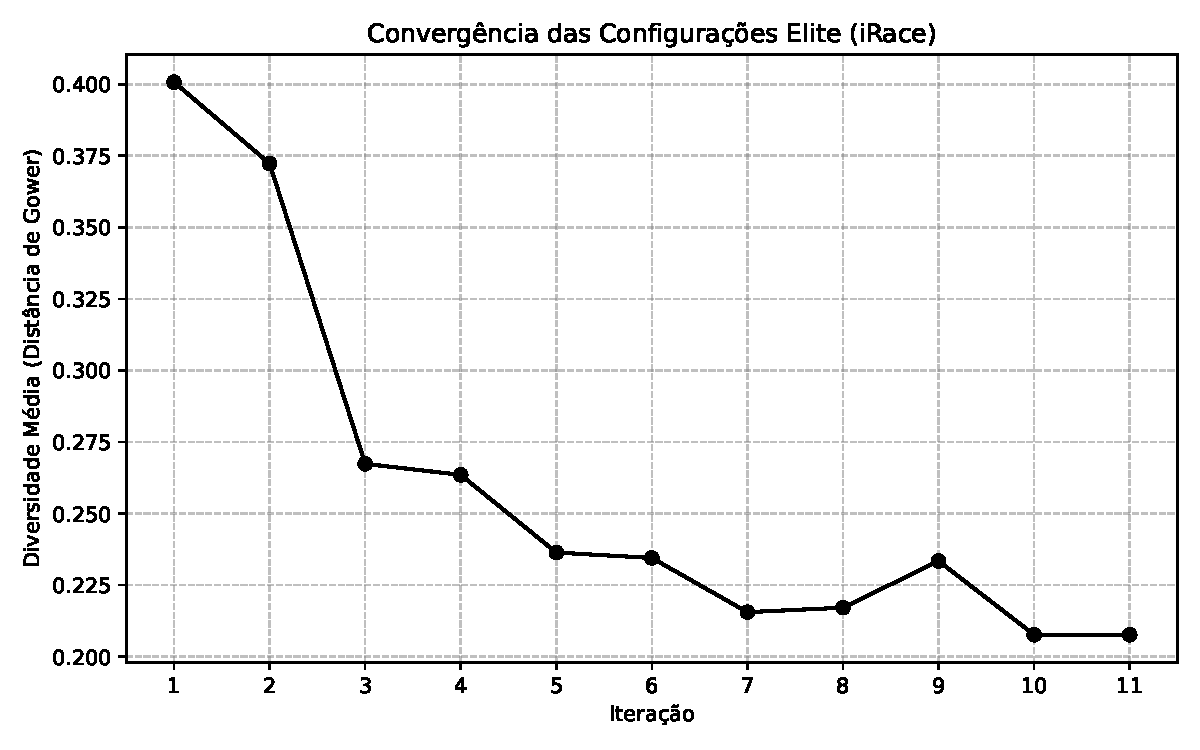
\includegraphics[width=0.9\linewidth]{img/grafico_convergencia.pdf}
    \caption*{\small \textbf{Fonte:} Os Autores.}
\end{figure}

O gráfico da Figura \ref{img:grafico_variancia} demonstra a redução progressiva da variância entre as configurações elite ao longo das iterações. Nesse sentido, a estabilização da variância na segunda metade do processo confirma a convergência do modelo de parâmetros para uma região de consenso, indicando que o processo de exploração atingiu maturidade no espaço de projeto.

Antes mesmo de realizar qualquer teste com as configurações elite, a análise das configurações elite permite a correlação direta com a literatura de \ac{JITJSS}. Por exemplo, a seleção de múltiplas vizinhanças no processo de busca. O processo de configuração pelo \textit{irace} ratifica a eficácia dessa estratégia, corroborando as abordagens de \cite{ahmadian2021meta} e \cite{wang2014variable}. Este cenário fornece um forte indício de que a exploração via vizinhança única é insuficiente diante da dificuldade do problema.

Além disso, diferentemente dos trabalhos citados, o presente trabalho propõe arquiteturas baseadas em uma Busca Tabu Iterada. Ou seja, o processo de configuração identificou que a integração de mecanismos tabu proporciona ganhos de desempenho à busca, mesmo em estruturas de múltiplas vizinhanças.

A predominância da solução inicial via \ac{GT}, associada à regra \texttt{edd}, reafirma a robustez desta combinação para o \ac{JITJSS}.

\subsection{Teste das configurações}

A convergência do processo de configuração para um grupo de algoritmos com características análogas fundamenta a etapa de testes em instâncias da literatura e a posterior comparação com o estado da arte. Para isso, a métrica de qualidade para cada instância consiste no desvio percentual em relação ao melhor valor conhecido da instância, conforme estabelecido pela Equação \ref{eq:desv_percent}. Nela, $S$ corresponde ao nosso resultado e $M$ ao melhor resultado conhecido para a instância. Ou seja, nesta escala, valores positivos indicam desempenho inferior à literatura, enquanto valores negativos apontam a superação dos marcos registrados.

\begin{equation} \label{eq:desv_percent}
     \frac{S-M}{M} * 100
\end{equation}

O procedimento inicial envolve a aplicação das configurações elite sobre o conjunto de teste. Por conta dos componentes estocásticos presentes nos algoritmos, geramos 5 \textit{seeds} aleatórias e realizamos a execução de cada configuração 5 vezes em cada instância, utilizando uma \textit{seed} diferente em cada execução.

% A distinção entre as instâncias de treinamento e de teste implica que a performance superior no primeiro conjunto não garante a liderança absoluta no segundo, fenômeno ilustrado na Tabela \ref{tab:results_confs}.
A Tabela \ref{tab:results_confs} contém um resumo do desempenho de cada configuração elite em comparação com o estado da arte. Cada coluna dessa tabela representa uma das configurações elite e as linhas contém: o número de instâncias nas quais o melhor resultado entre as cinco execuções é igual ou melhor ao estado da arte e o número de instâncias nas quais a mediana entre as cinco execuções é melhor ou igual ao estado da arte.
% Embora a configuração C1 tenha liderado o ranking no conjunto de treinamento, a C5 demonstrou maior capacidade de generalização ao atingir o maior volume de resultados iguais ou superiores ao estado da arte no conjunto de teste (34 instâncias no total).
Com isso, como representado na tabela, a configuração C1 demonstrou maior capacidade de generalização ao atingir o maior volume de resultados melhores ou iguais ao estado da arte no conjunto de teste (52 instâncias no total).

\begin{table}[ht]
\centering
\caption{Resumo dos resultados das configurações elite.}
\label{tab:results_confs}
% Substituímos tabular por tabularx e \resizebox por \textwidth
\begin{tabularx}{\textwidth}{Xcccccc}
\hline
\textbf{Parâmetro} & \textbf{C1} & \textbf{C2} & \textbf{C3} & \textbf{C4} & \textbf{C5} \\ \hline
Número de instâncias nas quais a melhor das soluções geradas pela configuração C1 é melhor ou igual ao estado da arte & 52 & 48 & 47 & 43 & 48  \\ 
Número de instâncias nas quais a mediana das soluções geradas pela configuração C1 é melhor ou igual ao estado da arte & 32 & 26 & 30 & 32 & 28  \\ 
\hline
\end{tabularx}
\caption*{\small \textbf{Fonte:} Os Autores.}
\end{table}

Dada a equivalência de desempenho entre os indivíduos elite, as análises subsequentes concentram-se na configuração C1. As tabelas \ref{tab:results_10}, \ref{tab:results_15} e \ref{tab:results_20} detalham os resultados para instâncias de 10, 15 e 20 tarefas, respectivamente, estabelecendo o comparativo com os resultados da literatura. Essas tabelas identificam as instâncias na primeira coluna e cada uma das colunas subsequentes contém os resultados dos diferentes trabalhos que compõem o estado da arte. Por fim, as duas últimas colunas representam os resultados do presente trabalho de forma que $B$ representa o melhor resultado obtido entre cinco execuções da configuração e a coluna $M$ representa a mediana dos resultados obtidos entre cinco execuções. Os resultados que representam o melhor valor encontrada para a respectiva instância são destacados em negrito nessas tabelas.

\begin{table}
\centering
\caption{Resultados da configuração C1 para as instâncias de teste de 10 tarefas.}
\label{tab:results_10}
\resizebox{\textwidth}{!}{
\begin{tabular}{lcccccccc}
\hline
\textbf{Instância}                & \textbf{Cplex}           & \textbf{[1]}          & \textbf{[2]}            & \textbf{[3]}        & \textbf{[4] }      & \textbf{[5]}        & \textbf{$B$} & \textbf{$M$}  \\
\hline
loose-equal-1-10x2  & \textbf{224,84} & \textbf{224,84} & \textbf{224,84} & \textbf{224,84} & \textbf{224,84} & \textbf{224,84}    & \textbf{224,84}       & \textbf{224,84}         \\
loose-equal-2-10x2  & \textbf{319,37} & 324,43          & \textbf{319,37} & \textbf{319,37} & \textbf{319,37} & \textbf{319,37}    & \textbf{319,37}       & \textbf{319,37}         \\
loose-equal-1-10x5  & 1738,05         & 1733,38         & 1738,05         & \textbf{1719,63} & 1725,16         & \textbf{1719,63}  & \textbf{1719,63}      & 1738,63                \\
loose-equal-2-10x5  & 971,96          & 968,89          & \textbf{967,73} & \textbf{967,73} & 968,05          & \textbf{967,73}    & \textbf{967,63}       & \textbf{967,73}                  \\
loose-equal-1-10x10 & 360,74          & 366,77          & 365,81          & 364,39          & 360,56          & \textbf{360,33}    & 360,74                & 364,59                  \\
loose-equal-2-10x10 & 251,86          & \textbf{249,85} & 252,99          & \textbf{249,85} & \textbf{249,85} & \textbf{249,85}    & \textbf{249,85}       & \textbf{249,85}         \\
loose-tard-1-10x2   & \textbf{416,44} & \textbf{416,44} & \textbf{416,44} & \textbf{416,44} & \textbf{416,44} & \textbf{416,44}    & \textbf{416,44}       & \textbf{416,44}         \\
loose-tard-2-10x2   & \textbf{137,94} & \textbf{137,94} & \textbf{137,94} & \textbf{137,94} & \textbf{137,94} & \textbf{137,94}    & \textbf{137,94}       & \textbf{137,94}         \\
loose-tard-1-10x5   & 176,83          & \textbf{175,08} & \textbf{175,08} & \textbf{175,08} & \textbf{175,08} & \textbf{175,08}    & \textbf{175,08}       & \textbf{175,08}                  \\
loose-tard-2-10x5   & 492,05          & 525,88          & 499,93          & \textbf{485,06} & 488,6           & 486,93             & \textbf{485,06}       & \textbf{485,06}         \\
loose-tard-1-10x10  & 375,71          & 383,84          & 380,26          & \textbf{374,2}  & \textbf{374,2}  & 375,58             & \textbf{374,2}        & 386,4                  \\
loose-tard-2-10x10  & \textbf{144,94} & \textbf{144,94} & 144,99          & \textbf{144,94} & \textbf{144,94} & \textbf{144,94}    & \textbf{144,94}       & \textbf{144,94}         \\
tight-equal-1-10x2  & \textbf{461,96} & \textbf{461,96} & \textbf{461,96} & \textbf{461,96} & \textbf{461,96} & \textbf{461,96}    & \textbf{461,96}       & \textbf{461,96}         \\
tight-equal-2-10x2  & \textbf{448,32} & \textbf{448,32} & \textbf{448,32} & \textbf{448,32} & \textbf{448,32} & \textbf{448,32}    & \textbf{448,32}       & \textbf{448,32}         \\
tight-equal-1-10x5  & \textbf{689,11} & \textbf{689,11} & \textbf{689,11} & \textbf{689,11} & \textbf{689,11} & \textbf{689,11}    & \textbf{689,11}       & 690,29                  \\
tight-equal-2-10x5  & \textbf{763,24} & 770,49          & 764,03          & \textbf{763,24} & \textbf{763,24} & \textbf{763,24}    & \textbf{763,24}       & \textbf{763,24}         \\
tight-equal-1-10x10 & 1281,66         & \textbf{1276,23} & 1277,44         & \textbf{1276,23} & \textbf{1276,23} & 1279,82         & 1281,66      & 1301,46                 \\
tight-equal-2-10x10 & 1885,25         & 1885,25         & 1871,23         & 1866,92         & 1865,94 & 1886,93                    & \textbf{1865,93}      & 1873,64                 \\
tight-tard-1-10x2   & \textbf{179,46} & \textbf{179,46} & \textbf{179,46} & \textbf{179,46} & \textbf{179,46} & \textbf{179,46}    & \textbf{179,46}       & \textbf{179,46}         \\
tight-tard-2-10x2   & \textbf{145,37} & \textbf{145,37} & \textbf{145,37} & \textbf{145,37} & \textbf{145,37} & \textbf{145,37}    & \textbf{145,37}       & \textbf{145,37}         \\
tight-tard-1-10x5   & \textbf{379,19} & 380,82          & 380             & \textbf{379,19} & \textbf{379,19} & \textbf{379,19}    & 386,57                & 389,43                  \\
tight-tard-2-10x5   & 635,93          & \textbf{627,45} & 628,68          & \textbf{627,45} & 628,02          & \textbf{627,45}    & \textbf{627,45}       & \textbf{627,45}         \\
tight-tard-1-10x10  & 687,65          & 717,85          & 746,03          & 668,14          & \textbf{667,97} & 669,15             & 669,93                & 687,65                  \\
tight-tard-2-10x10  & 779,17          & 780,82          & 785,79          & \textbf{777,85} & 778,32          & 780,74             & 780,66                & 804,23                  \\
\hline
\end{tabular}
}
\caption*{\small \textbf{Fonte:} A coluna Cplex foi retirada de \cite{ahmadian2021meta} e cada coluna numerada representa os resultados de um trabalho: \textbf{[1]} \cite{dos2010combination}, \textbf{[2]} \cite{wang2014variable}, \textbf{[3]} \cite{ahmadian2021meta}, \textbf{[4]} \cite{abderrazzak2022adaptive} e \textbf{[5]} \cite{sabri2023reinforcement}.}
\end{table}


\begin{table}
\centering
\caption{Resultados da configuração C1 para as instâncias de teste de 15 tarefas.}
\label{tab:results_15}
\resizebox{\textwidth}{!}{
\begin{tabular}{lcccccccc}
\hline
\textbf{Instância}                & \textbf{Cplex}           & \textbf{[1]}          & \textbf{[2]}            & \textbf{[3]}        & \textbf{[4] }      & \textbf{[5]}        & \textbf{$B$} & \textbf{$M$}   \\
\hline
loose-equal-1-15x2  & \textbf{1041,33} & \textbf{1041,33} & \textbf{1041,33} & \textbf{1041,33} & \textbf{1041,33} & \textbf{1041,33} & \textbf{1041,33}    & \textbf{1041,33}  \\
loose-equal-2-15x2  & \textbf{497,97}  & \textbf{497,97}  & 514,72          & 512,54          & \textbf{497,97}  & \textbf{497,97}    & \textbf{497,97}     & 505,16           \\
loose-equal-1-15x5  & 3457,57         & 3220,16         & 3321,54         & 3272,46         & 3258,72         & 3229,16               & \textbf{3196,85}    & 3247,89  \\
loose-equal-2-15x5  & 3437,32         & 3328,86         & 3310,27         & 3260,81         & 3255,13         & \textbf{3251,84}      & 3274,38             & 3290,70                 \\
loose-equal-1-15x10 & \textbf{875,74}  & 1008,28         & 977,43          & 906,49          & 897,51          & 913,26               & 898,99              & 938,80                \\
loose-equal-2-15x10 & 1587,09         & 1720,18         & 1584,44         & \textbf{1487,33} & 1538,27         & 1492,11              & 1554,18             & 1594,60                \\
loose-tard-1-15x2   & \textbf{654,84}  & \textbf{654,84}  & \textbf{654,84}  & \textbf{654,84}  & \textbf{654,84}  & \textbf{654,84}  & \textbf{654,84}     & \textbf{654,84}   \\
loose-tard-2-15x2   & 293,17          & \textbf{279,71}  & 297,54          & 285,16          & 289,36          & \textbf{279,71}      & \textbf{279,71}     & 290,88           \\
loose-tard-1-15x5   & 1281,87         & 1320,93         & 1315,47         & 1281    & 1292,28         & 1317,56                       & \textbf{1280,74}    & 1281,41          \\
loose-tard-2-15x5   & 335,55          & 329,47          & 335,55          & 328,26  & 330,14          & 332,25                        & \textbf{327,60}     & 328,88           \\
loose-tard-1-15x10  & \textbf{277}     & 297,19          & 296,6           & \textbf{277}     & \textbf{277}     & \textbf{277}       & 281,45              & 287,03              \\
loose-tard-2-15x10  & 597,93  & 713,97          & 664,13          & 601,24          & 627,81          & 603,67                        & \textbf{587,24}     & \textbf{592,31}         \\
tight-equal-1-15x2  & 3366,66         & \textbf{3344,54} & \textbf{3344,54} & \textbf{3344,54} & \textbf{3344,54} & \textbf{3344,54}  & \textbf{3344,54}    & \textbf{3344,54}   \\
tight-equal-2-15x2  & \textbf{1479,76} & \textbf{1479,76} & \textbf{1479,76} & \textbf{1479,76} & \textbf{1479,76} & \textbf{1479,76} & \textbf{1479,76}    & \textbf{1479,76}   \\
tight-equal-1-15x5  & 1412,71         & 1369,06         & 1345,21         & 1342,3          & 1343,08         & 1345,18               & \textbf{1318,68}    & \textbf{1318,68}   \\
tight-equal-2-15x5  & 2782,17         & 2630,06         & 2709,13         & 2641,28         & \textbf{2563,16} & 2602,99               & 2626,67             & 2651,16           \\
tight-equal-1-15x10 & 7167,59         & 7380,76         & 8120,43         & 6820,87         & 6811,54 & 7115,63                       & \textbf{6610,44}    & \textbf{6748,88}           \\
tight-equal-2-15x10 & 5407,42         & 4893,44         & 4966,34         & 4760,48         & 4801,47         & 4757,06                & \textbf{4652,41}    & \textbf{4730,08}    \\
tight-tard-1-15x2   & 806,92          & \textbf{790,5}   & 790,66          & \textbf{790,5}   & \textbf{790,5}   & \textbf{790,5}     & \textbf{790,5}      & \textbf{790,5}       \\
tight-tard-2-15x2   & \textbf{905,37}  & \textbf{905,37}  & \textbf{905,37}  & \textbf{905,37}  & \textbf{905,37}  & \textbf{905,37}   & \textbf{905,37}     & \textbf{905,37}      \\
tight-tard-1-15x5   & 1371,29         & 1371,37         & 1426,97         & 1359,18         & 1366,45         & \textbf{1341,69}       & 1358,21             & 1359,18            \\
tight-tard-2-15x5   & 721,46          & 691,1           & 725,72          & 681,27          & 677,8           & 695,08                 & \textbf{677,57}     & 681,62     \\
tight-tard-1-15x10  & 815,03          & 800,87          & 832,08          & 767,26  & 770,91          & 775,4                          & \textbf{757,83}     & 785,75        \\
tight-tard-2-15x10  & 1267,53         & 1310,04         & 1452,9          & 1224,82         & 1243,52         & 1226,23                & \textbf{1170,94}    & \textbf{1172,30}     \\
\hline
\end{tabular}
}
\caption*{\small \textbf{Fonte:} A coluna Cplex foi retirada de \cite{ahmadian2021meta} e cada coluna numerada representa os resultados de um trabalho: \textbf{[1]} \cite{dos2010combination}, \textbf{[2]} \cite{wang2014variable}, \textbf{[3]} \cite{ahmadian2021meta}, \textbf{[4]} \cite{abderrazzak2022adaptive} e \textbf{[5]} \cite{sabri2023reinforcement}.}
\end{table}

\begin{table}
\centering
\caption{Resultados da configuração C1 para as instâncias de teste de 20 tarefas.}
\label{tab:results_20}
\resizebox{\textwidth}{!}{
\begin{tabular}{lcccccccc}
\hline
\textbf{Instância}                & \textbf{Cplex}           & \textbf{[1]}          & \textbf{[2]}            & \textbf{[3]}        & \textbf{$B$} & \textbf{$M$}   \\
\hline
loose-equal-1-20x2  & 2565,51 & \textbf{2548,95} & 2551,22 & \textbf{2548,95}                   & \textbf{2548,95}     & 2549,19               \\
loose-equal-2-20x2  & 3105,34 & \textbf{3069,13} & 3070,16 & \textbf{3069,13} & \textbf{3069,13}     & \textbf{3069,13}               \\
loose-equal-1-20x5  & 8271,34 & 7545,44 & 7758,02 & 7524,13                   & \textbf{7487,77}     & 7666,29              \\
loose-equal-2-20x5  & 7793,45 & 7252,81 & 7302,01 & 7059,38                   & \textbf{7022,53}     & 7128,87               \\
loose-equal-1-20x10 & 5597,4  & 5260,48 & 5476,47 & 4651,31                   & \textbf{4592,02}     & 4687,60               \\
loose-equal-2-20x10 & 1862,41 & 1987,65 & 1718,08 & \textbf{1597,89}          & 1608,61              & 1701,42                        \\
loose-tard-1-20x2   & 1265,36 & 1206,97 & 1205,59 & 1206,4                     & \textbf{1203,88}     & 1206,97               \\
loose-tard-2-20x2   & 772,89  & \textbf{769,35}  & 790,12 & \textbf{769,35}   & 771,06               & 776,01                          \\
loose-tard-1-20x5   & 3548,14 & 2938,24 & 3517,2  & \textbf{2931,11}          & 2936,63              & 3068,78                         \\
loose-tard-2-20x5   & 4048,77 & 3722,61 & 3684,67 & 3627,51                   & \textbf{3617,49}     & 3646,58               \\
loose-tard-1-20x10  & 6494,34 & 5093,89 & 5478,21 & 4817,32                   & \textbf{4789,13}     & 5114,72               \\
loose-tard-2-20x10  & 1545,95 & 1570,64 & 1599,55 & \textbf{1401,28}          & 1516,95              & 1531,54                         \\
tight-equal-1-20x2  & 1940,06 & 1937,49 & 1939,11 & 1936,45                   & \textbf{1933,72}     & \textbf{1933,72}               \\
tight-equal-2-20x2  & 961,44  & \textbf{941,69}  & 959,65  & 943,7            & 944,93               & 948,01                          \\
tight-equal-1-20x5  & 3013,79 & 2866,94 & 2935,95 & 2865,95                   & \textbf{2821,02}     & \textbf{2865,45}               \\
tight-equal-2-20x5  & 7233,35 & 6741,16 & 6964,91 & 6613,62                   & \textbf{6581,72}     & 6626,55               \\
tight-equal-1-20x10 & 11561,7 & 10607,2 & 11073,1 & \textbf{10378,8}          & 10534,50             & 10831,90                          \\
tight-equal-2-20x10 & 8501,42 & 7310,32 & 7317,74 & \textbf{6839,3}           & 6892,16              & 7047,16                          \\
tight-tard-1-20x2   & 1675,37 & \textbf{1671,87} & 1682,94 & 1674,6           & \textbf{1671,87}     & 1672,03               \\
tight-tard-2-20x2   & 1489,65 & \textbf{1448,66} & 1459,57 & 1451,61          & \textbf{1448,66}     & \textbf{1448,66}               \\
tight-tard-1-20x5   & 3821,29 & 3672,18 & 3669,09 & 3620,61                   & \textbf{3598,12}     & \textbf{3618,13}               \\
tight-tard-2-20x5   & 1881,02 & 1858,19 & 1976,11 & \textbf{1792,78}          & 1802,78              & 1808,36                         \\
tight-tard-1-20x10  & 4984,31 & 4853,81 & 5536,64 & 4445,59                   & \textbf{4406,01}     & \textbf{4434,02}               \\
tight-tard-2-20x10  & 4057,01 & 3358,61 & 3245,9  & \textbf{3085,54}          & 3207,33              & 3242,14                         \\
\hline
\end{tabular}
}
\caption*{\small \textbf{Fonte:} A coluna Cplex foi retirada de \cite{ahmadian2021meta} e cada coluna numerada representa os resultados de um trabalho: \textbf{[1]} \cite{dos2010combination}, \textbf{[2]} \cite{wang2014variable} e \textbf{[3]} \cite{ahmadian2021meta}.}
\end{table}

A análise dos dados revela que o algoritmo configurado igualou ou superou o estado da arte em aproximadamente 72,2\% das 72 instâncias de teste. Essa eficácia concentra-se predominantemente nas instâncias de 10 tarefas, nas quais o algoritmo atingiu o marco de 83\% de sucesso em relação aos melhores valores da literatura. Além disso, a análise das medianas corrobora a robustez da configuração C1, a qual igualou ou superou os marcos bibliográficos em 44,4\% das instâncias.
% a configuração C5 obteve melhorias incrementais em casos específicos. Nesse sentido, a hipótese central reside na proximidade desses resultados em relação ao limite inferior de otimalidade, especialmente nos cenários de menor escala, o que restringe o potencial de ganho de novas heurísticas..

Os dados expostos indicam uma redução gradual na eficácia da mediana conforme a escala das instâncias aumenta. Contudo, o desvio médio das medianas em relação às melhores soluções individuais é de apenas 1,06\%, evidenciando a estabilidade do método estocástico frente a variações de sementes aleatórias.

Embora os marcos de desempenho demonstrem competitividade, a análise prévia baseia-se no melhor valor conhecido para cada instância. Esta métrica representa um limite superior composto pelos melhores resultados de todos os trabalhos da literatura combinados. Dessa forma, a comparação individual apresentada na Tabela \ref{tab:comparacao_estado} isola o desempenho da proposta frente a cada método do estado da arte de maneira independente. As colunas organizam os resultados por autor, enquanto as linhas quantificam o número de instâncias nas quais a configuração C1 obteve desempenho igual ou superior ao de cada método de referência. Com isso, os resultados evidenciam que a configuração gerada por este estudo apresenta qualidade superior em comparações diretas com cada trabalho da literatura.

\begin{table}[ht]
\centering
\caption{Comparação individual entre este trabalho e algoritmos da literatura.}
\label{tab:comparacao_estado}
\begin{tabularx}{\textwidth}{Xcccccc}
\hline
\textbf{}                 & \textbf{[1]}          & \textbf{[2]}            & \textbf{[3]}        & \textbf{[4] }      & \textbf{[5]}   \\ \hline
Porcentagem das instâncias nas quais a melhor das soluções geradas pela configuração C1 é melhor ou igual aos resultados de um trabalho & 94,44 & 97,22 & 77,77 & 79,16 & 81,25  \\ 
Porcentagem das instâncias nas quais a mediana das soluções geradas pela configuração C1 é melhor ou igual aos resultados de um trabalho & 75 & 88,88 & 50 & 62,5 & 62,5  \\ 
\hline
\end{tabularx}
\caption*{\small \textbf{Fonte:} cada coluna numerada representa os resultados de um trabalho: \textbf{[1]} \cite{dos2010combination}, \textbf{[2]} \cite{wang2014variable}, \textbf{[3]} \cite{ahmadian2021meta}, \textbf{[4]} \cite{abderrazzak2022adaptive} e \textbf{[5]} \cite{sabri2023reinforcement}.}
\end{table}

Como mencionado anteriormente, todas as execuções do algoritmo levam 60 segundos. O algoritmo de \ac{ILS} opera sem mecanismos de detecção de convergência das soluções, gastando o tempo limite de 60 segundos em todas as execuções. Entretanto, a localização da solução final ocorre, em média, aos 21,1 segundos de execução. Em instâncias de 10 tarefas, este marco reduz-se para 9 segundos. Esses indicadores sugerem que a integração de critérios de convergência otimizará a eficiência computacional do algoritmo, permitindo a obtenção de resultados da mesma qualidade em frações do tempo total estabelecido.

